%% ============================================================
%%  APA7-style manuscript draft
%%  Adjective Ordering in Referential Communication
%% ============================================================
\documentclass[man,floatsintext]{apa7}
\setcounter{secnumdepth}{3}

% ---- packages ---------------------------------------------------------------
\usepackage[american]{babel}
\usepackage[T1]{fontenc}
\usepackage[utf8]{inputenc}
\usepackage{microtype}
\usepackage{booktabs}
\usepackage{tabularx}
\usepackage{multirow}
\usepackage{amsmath, amssymb}
\usepackage{mathtools}
\usepackage{stmaryrd}
\usepackage{bm}
\usepackage{graphicx}
\graphicspath{{10-writing/figures/}{figures/}}
\usepackage{float}
\usepackage{cleveref}
\usepackage{todonotes}
\presetkeys{todonotes}{inline, backgroundcolor=yellow!40}{}
\usepackage[natbibapa]{apacite}

% ---- convenience commands ---------------------------------------------------
\newcommand{\eg}{\textit{e.g.}}
\newcommand{\ie}{\textit{i.e.}}
\newcommand{\adj}[1]{\textsc{#1}}
\newcommand{\utter}[1]{\textsf{#1}}
\newcommand{\param}[1]{\ensuremath{#1}}

% ---- title matter -----------------------------------------------------------
\shorttitle{Adjective Ordering in Referential Communication}
\title{Adjective Ordering in Referential Communication:\\
Subjectivity, Discriminatory Strength, and Incremental Pragmatics}
\authorsnames{Hening Wang, Fabian Schlotterbeck, and Michael Franke}
\authorsaffiliations{University of T\"ubingen}
\leftheader{Wang et al.}

\abstract{Adjective ordering preferences are robust across languages, and recent work suggests that they reflect both stable lexical-semantic asymmetries and context-sensitive pressures on efficient reference resolution.
The present paper develops a Rational Speech Act model that brings these traditions together by crossing two dimensions in a $2 \times 2$ comparison: speaker architecture (global vs.\ incremental) and semantic regime (context-fixed vs.\ context-updating).
Under context-updating semantics, the interpretation of a gradable adjective is recomputed from the listener's running posterior during composition, making adjective order non-commutative; under context-fixed semantics, interpretations are fixed from the scene.
Two referential experiments in German provide the empirical target: a slider-rating study that measures graded preference for competing adjective orders and a free-production study that measures actual utterance choice.
Across both experiments, ordering preferences vary systematically with the discriminatory value of the adjectives in the current scene, with speakers tending to place the more discriminating adjective earlier in the string, while still preserving a baseline size-first tendency.
Bayesian model comparison shows that incremental production is the dominant mechanism across both datasets.
In the production data, context-updating semantics provides a significant further improvement, but only when paired with an incremental speaker --- an interaction indicating that the two mechanisms are synergistic.
For free production over the full inventory of adjective strings, this comparison is run on an incremental speaker developed and selected to fit that richer response space.
Simulation results confirm that a substantial baseline ordering effect already follows from context-sensitive restrictive composition alone.
We argue that adjective ordering in referential communication is best understood as a graded adaptation to efficient, incremental reference resolution: subjectivity provides a baseline bias, discriminatory strength modulates that bias in context, and incremental production with context-updating semantics best captures how speakers realize these pressures online.}

\keywords{adjective ordering, Rational Speech Act, incremental pragmatics, communicative efficiency, subjectivity}

% =============================================================================
\begin{document}
\maketitle

% =============================================================================
\section{Introduction}
\label{sec:intro}
% =============================================================================

When multiple adjectives modify a noun, speakers across typologically diverse languages prefer similar orderings --- ``big brown bag'' over ``brown big bag'' \citep{scontras2023adjective,sproat1991}.
Previous research (for an overview, see \citealp{scontras2023adjective}) has linked these preferences to meaning-based factors such as closeness to the noun and inherentness \citep{sweet1898,whorf1945grammatical,martin1969a}, to class-based hierarchies \citep{quirk1972,dixon1982,cinque1994,scott2002}, and to information-theoretic measures \citep{Hahn_information_2018,futrell-etal-2020-determines,dyer2023evaluating}.
However, no single factor has proven sufficient; even the best individual predictors leave complementary variance unexplained \citep{dyer2023evaluating}.
Furthermore, the preferences are context-sensitive in ways that fixed hierarchies do not fully capture \citep{trotzke2019,fukumura2018ordering}.

We focus on two lines of recent work that ground ordering preferences in communicative efficiency.
\citet{scontras2017subjectivity} showed that \emph{subjectivity} is a strong predictor of preferred adjective distance from the noun, and subsequent work argued that this regularity follows from restrictive composition and sequential context update: less subjective adjectives contribute more useful information at the inner, more restricted stage of modification \citep{franke2019subjectivity,scontras2019grammatical,scontras2020incremental}.
Separately, \citet{fukumura2018ordering} demonstrated that speakers in referential tasks tend to place the more \emph{discriminating} adjective first, maximising informativeness in the given context, and \citet{rubio2021wordorder} generalised this into an \emph{incremental efficiency} hypothesis: the utility of a modifier should be evaluated at the point in the utterance where it is encountered, not only after the full description has been heard.

Both lines of work appeal to communicative efficiency, but they locate it at different levels --- one in the compositional semantics, the other in the online production process.
The central question of this paper is how these two levels interact.
Subjectivity provides a stable ordering bias, but the communicative context determines how strongly that bias is expressed in a particular scene.
When one property suffices for identification and another does not, the more useful property may exert pressure for earlier mention even when it conflicts with the canonical order.
What is missing is a unified account that separates the contribution of stable compositional asymmetries from context-sensitive, online production pressures and tests whether these mechanisms are independently additive or synergistic.

We address three questions.
First, can canonical ordering preferences already arise from \emph{context-sensitive restrictive composition} without an incremental production mechanism?
Second, does an explicitly \emph{incremental} speaker --- one that chooses modifiers word by word --- add explanatory value beyond a global, utterance-level evaluation?
Third, does \emph{context-updating semantics}, in which the meaning of a gradable adjective is recomputed from the listener's running posterior, provide a further benefit --- and is that benefit contingent on incremental production?

To answer these questions, we develop a Rational Speech Act (RSA) model \citep{goodman2016pragmatic,degen2023rational} that crosses two dimensions in a $2 \times 2$ comparison: \emph{speaker architecture} (global vs.\ incremental) and \emph{semantic regime} (context-fixed vs.\ context-updating).
The global speaker evaluates complete utterances; the incremental speaker chooses one modifier at a time.
Under context-updating semantics, the interpretation of ``big'' depends on what the listener already believes after hearing earlier words, so that ``big blue'' and ``blue big'' need not be equivalent; under context-fixed semantics, the size threshold is determined once from the scene.
All four model variants are fitted to data from two complementary referential experiments in German --- a slider-rating study measuring graded ordering preferences and a constrained production study measuring actual utterance choice --- in a shared paradigm that varies discriminatory strength across scenes.
Model comparison uses Bayesian leave-one-out cross-validation \citep[PSIS-LOO;][]{vehtari2017practical}, which quantifies how much predictive accuracy each mechanism adds and detects their interaction.
A simulation study complements the empirical work by crossing both speaker architectures with both semantic regimes to identify which ordering effects require context-sensitive composition, which require incremental production, and which emerge only from their interaction.

Both experiments confirm that ordering preferences vary systematically with discriminatory strength: speakers tend to place the more informative adjective earlier while preserving a baseline size-first tendency.
The simulation shows that recursive semantics is necessary for the baseline size-first advantage: the global speaker produces the canonical ordering only under context-updating semantics, where threshold adaptation makes the two orderings informationally non-equivalent.
In the model comparison, incremental production emerges as the dominant mechanism across both datasets.
In the production data, context-updating semantics provides a significant further improvement, but only when paired with an incremental speaker --- an interaction indicating that the two mechanisms are synergistic.
\Cref{fig:overview} provides a schematic overview of the modelling framework, experiments, and key findings.
We introduce the framework conceptually in \Cref{sec:framework}, before the experiments, and defer its formal specification to \Cref{sec:model}.

\begin{figure}[htbp]
  \centering
  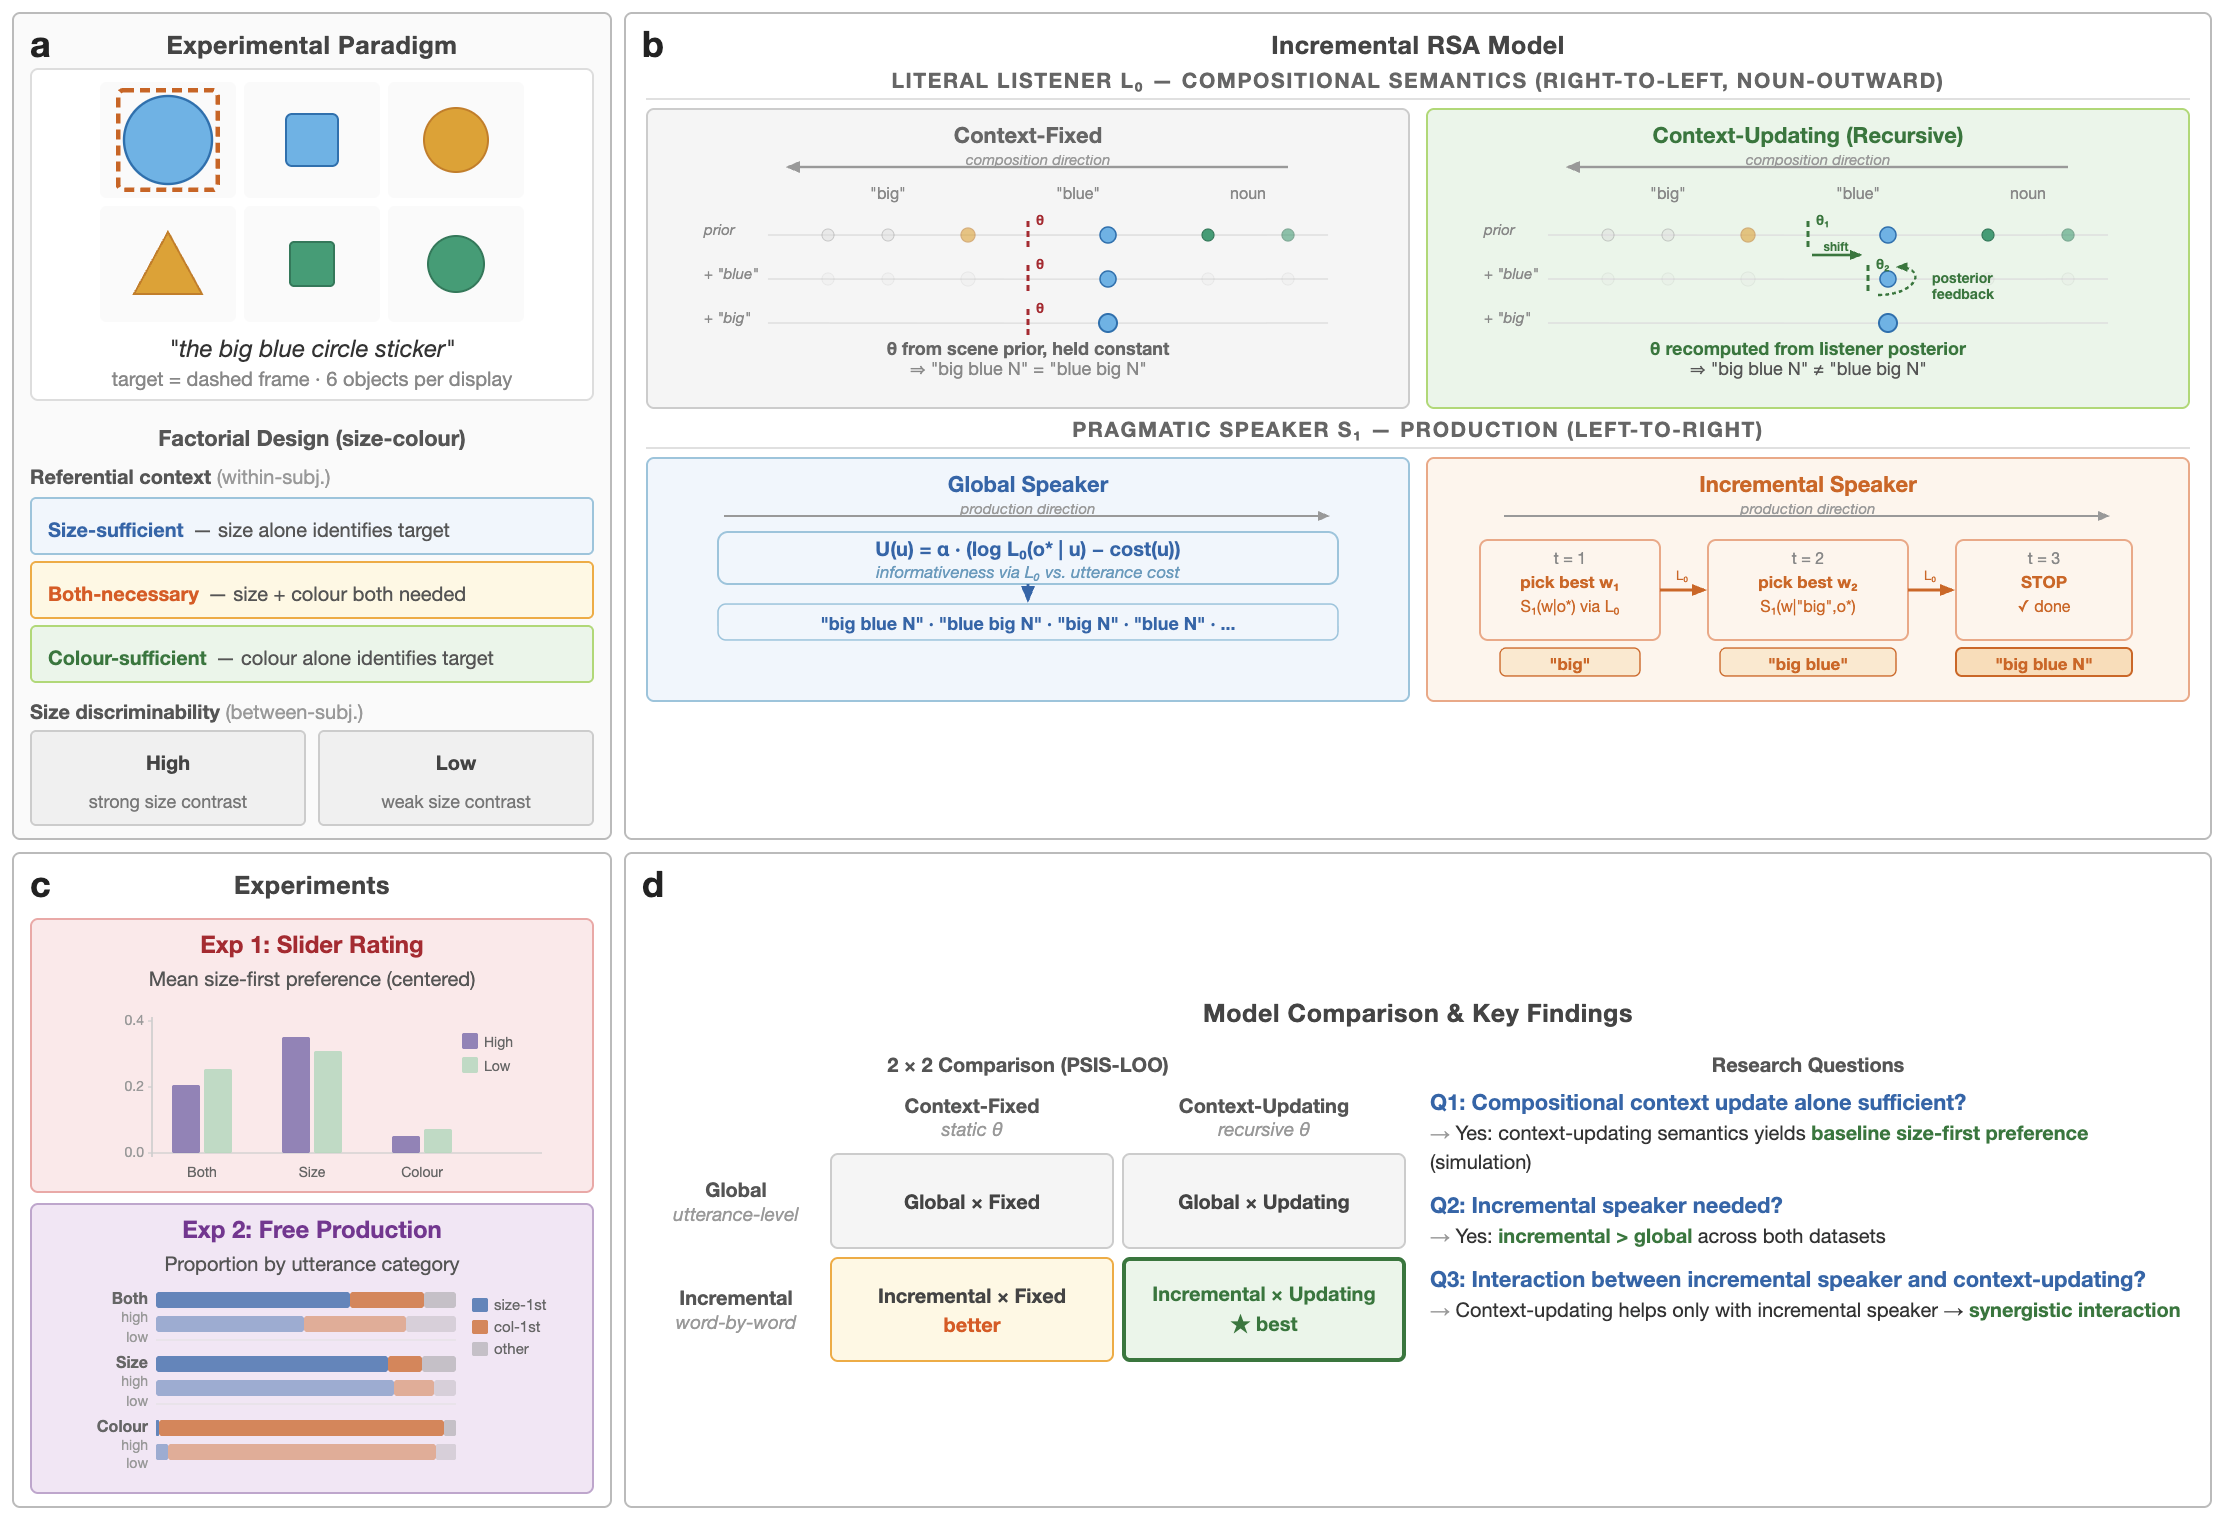
\includegraphics[width=\textwidth]{overview_figure.png}
  \caption{Overview of the present study.
  (\textbf{a})~Experimental paradigm: six-object displays varying in referential context (within-subj.) and size discriminability (between-subj.).
  (\textbf{b})~The RSA model crosses two dimensions: compositional semantics (context-fixed vs.\ context-updating $\theta$, right-to-left) and speaker architecture (global vs.\ incremental, left-to-right).
  (\textbf{c})~Empirical results: slider ratings of ordering preference and production proportions by utterance category.
  (\textbf{d})~$2 \times 2$ model comparison (PSIS-LOO) and key findings (Q1--Q3).}
  \label{fig:overview}
\end{figure}

% =============================================================================
\section{Background}
\label{sec:background}
% =============================================================================

Three lines of research bear on the question of how speakers choose and order adjectives, yet to date they have developed largely independently: subjectivity-based accounts trace canonical ordering preferences to compositional interpretation, efficiency-based accounts link adjective choice and order to the discriminatory strength covered by the referential context, and incremental pragmatic models formalize the word-by-word process through which speakers produce utterances.
The model developed in this paper integrates all three.

\subsection{Subjectivity and Adjective Ordering}
\label{sec:bg:subjectivity}

A central empirical generalization in the adjective-ordering literature is the relation between an adjective's \emph{subjectivity} and its preferred distance from the noun.
\citet{scontras2017subjectivity} operationalized subjectivity as susceptibility to faultless disagreement and showed that it explains a large share of variance in English ordering preferences, outperforming earlier predictors such as inherentness and intersectivity.
Subsequent cross-linguistic work suggests that this relationship is not peculiar to English, but reflects a broader regularity in adjective ordering \citep{trainin2021s,scontras2023adjective}.

\citet{scontras2019grammatical} argue that the explanatory core of this effect lies in restrictive composition.
Adjectives closer to the noun apply over a denotation that has already been narrowed by outer modifiers.
In such a restricted comparison class, a less subjective adjective is advantageous because its interpretation is more stable.
\citet{franke2019subjectivity} make the same intuition explicit in simulation, showing that subjectivity-aligned orders increase average communicative success under sequential composition with noisy meanings.
Crucially, this explanation does not require a word-by-word production mechanism; the ordering pressure can emerge from the compositional system itself.

That conclusion is strengthened by \citet{scontras2020incremental}, who argue that what matters is \emph{incremental semantic restriction}.
If nominal structure supports sequential narrowing of the comparison class, then subjectivity-based ordering pressures should arise even without an incremental speaker in the usual process-model sense.
This identifies a plausible minimal mechanism for canonical ordering: context-sensitive restrictive composition may already suffice to produce a baseline size-first tendency.

\subsection{Communicative Efficiency and Discriminatory Strength}
\label{sec:bg:efficiency}

The subjectivity account, however, addresses only one source of ordering pressure.
A separate line of work has shown that adjective use is sensitive to the demands of the immediate communicative context, including whether a modifier helps the listener identify the referent quickly and efficiently \citep{rubio2016redundant,rubio2019overinformative,degen2020redundancy}.
This literature treats adjective choice and adjective order as part of a broader problem of reference generation rather than as the expression of a static lexical hierarchy.

\citet{fukumura2018ordering} provide a direct precedent for the present experiments.
In their production studies, speakers were more likely to place the more discriminating adjective first, consistent with a \emph{discriminatory efficiency hypothesis}: order should reflect which property best distinguishes the target in the current scene.
This is a different source of pressure from subjectivity, because it is inherently local.
The same adjective may be highly useful in one display and much less useful in another.

Rubio-Fern\'andez and colleagues place this idea in a broader framework of \emph{incremental efficiency} \citep{rubio2020incrementality,rubio2021wordorder}.
Their central claim is that the efficiency of a referential expression should be evaluated as the utterance unfolds, not only after the full description has been heard.
From this perspective, word order matters because it determines how the listener's search space is narrowed over time.
Prenominal and postnominal systems therefore create different pragmatic affordances, and even redundant modifiers can be useful if they facilitate early search.
What matters is not merely whether a property contributes to unique reference in the end, but whether it has discriminatory value at the relevant stage of processing.

For the present paper, this distinction motivates the central empirical manipulation.
Within the modeled size--colour subset, the experiments vary whether size is sufficient, colour is sufficient, or whether both properties are necessary for identification, and they additionally vary how discriminable the size contrast is.
These manipulations operationalize the context-sensitive component of the theory: if adjective ordering is responsive to discriminatory strength, then preferences and production should shift with the referential scene rather than reflecting only a global size-first prior.

\subsection{Incremental Pragmatic Models}
\label{sec:bg:incremental}

The Rational Speech Act (RSA) framework offers a natural way of formalizing these pressures.
In RSA, a pragmatic speaker selects utterances by reasoning about a listener's posterior, and the listener in turn reasons about the speaker's choice \citep{goodman2016pragmatic}.
Although standard RSA treats complete utterances as the units of choice, the same logic can be defined incrementally, with the speaker choosing one word at a time on the basis of how each token updates the listener's beliefs \citep{cohngordon2019incremental}.
Existing incremental pragmatic models and related work on redundancy establish that word-by-word reasoning can capture asymmetries between adjective positions and between prenominal and postnominal systems \citep{degen2020redundancy,rubio2021wordorder}.
What these accounts usually do not assume is that lexical meanings themselves change as the listener's posterior changes.
In most such accounts the posterior updates online, but the interpretation of an adjective remains fixed relative to the scene.
\citet{schlotterbeck2023incremental} introduced an alternative in which the threshold for a gradable adjective is recomputed from the listener's current posterior at each stage of composition, together with the slider-rating paradigm that forms the basis for one of the experiments reported here.
That study showed that the model qualitatively captures both a subjectivity-driven baseline ordering and a discriminatory-strength modulation, but it did not isolate the respective contributions of incremental production and context-updating semantics, nor did it assess their quantitative fit.

% =============================================================================
\section{The Modelling Framework}
\label{sec:framework}
% =============================================================================

We extend \citet{schlotterbeck2023incremental} in four directions.
We embed the model in a systematic $2 \times 2$ comparison of speaker architecture and semantic regime, including a context-fixed ablation; we add a constrained production experiment that provides a richer response space; we introduce a simulation study that identifies which ordering effects follow from context-updating composition alone; and we use Bayesian model comparison to quantify each mechanism's contribution and to reveal an interaction that the earlier qualitative analysis could not detect.
Here we describe the framework at a conceptual level; the meaning functions, speaker definitions, and inference setup are given formally in \Cref{sec:model}.
The remaining subsections develop these components in turn.

\subsection{Reference, Scenes, and the Speaker's Problem}
\label{sec:framework:scene}

The model addresses a referential task.
A scene contains several objects that vary in size, colour, and form, and one of them is the intended referent --- in our materials, the largest object that matches the target colour and form.
A speaker must choose an adjective string that lets a listener identify this referent, and the listener interprets that string by progressively narrowing the set of objects it could pick out.
Because objects differ along three properties, the same referent can be described in many ways, and the order in which adjectives are produced is itself part of what the speaker chooses.

\subsection{Rational Speech Act Reasoning}
\label{sec:framework:rsa}

We model this choice within the Rational Speech Act framework, in which a pragmatic speaker selects utterances by reasoning about how a listener would interpret them, and the listener reasons recursively about the speaker.
A literal listener interprets an adjective by retaining the objects it applies to, and a pragmatic speaker prefers descriptions that make the intended referent easy to recover.
Determinate properties such as colour and form are treated as nearly categorical, whereas size is gradable: whether an object counts as ``big'' depends on the comparison class it is evaluated against, so the size term is informative only relative to the objects currently under consideration.

\subsection{Two Mechanisms for Order Sensitivity}
\label{sec:framework:mechanisms}

The framework isolates two ways in which adjective order can come to matter.
The first is the \emph{speaker architecture}.
A global speaker evaluates complete adjective strings and chooses among them as wholes, whereas an incremental speaker chooses one adjective at a time, weighing at each step how the next word would reshape the listener's beliefs.
Incremental choice makes the usefulness of a modifier depend on where it occurs in the string, not only on the description as a whole.
The second is the \emph{semantic regime}.
Under context-fixed semantics, the size threshold is computed once from the scene and held constant, so reordering the adjectives cannot change what ``big'' means.
Under context-updating semantics, the threshold is recomputed from the listener's running beliefs, so that once ``blue'' has restricted attention to blue objects, ``big'' is judged against just those objects; ``big blue'' and ``blue big'' can then differ even though they contain the same words.
This non-commutativity connects to \citeauthor{teodorescu2006}'s (\citeyear{teodorescu2006}) observation that ordering restrictions weaken precisely when the alternative orders are not truth-conditionally equivalent.

Crossing these two binary choices yields a $2 \times 2$ space of models --- speaker architecture (global vs.\ incremental) by semantic regime (context-fixed vs.\ context-updating).
We do not claim that production-level incrementality is required for adjective-ordering preferences in general; the subjectivity literature and our own simulations (\Cref{sec:simulation}) indicate that context-sensitive restrictive composition already accounts for much of the canonical tendency.
The question is how much explanatory work remains once that baseline is in place, and in particular whether incremental production and context-updating semantics are independently useful or interact.

\subsection{Qualitative Predictions}
\label{sec:framework:predictions}

This framework yields qualitative predictions that the two experiments are designed to test (\Cref{tab:predictions}).
Because the model retains a stable, subjectivity-aligned ordering prior, it predicts a baseline size-first preference that survives even when colour alone identifies the referent (P1).
Because the pragmatic component is sensitive to which property discriminates the referent in the current scene, it predicts that the size-first preference weakens as colour becomes the more useful property (P2).
The sharpness of the size contrast should act only as a secondary modulator, shifting preferences in interaction with referential context rather than as a strong main effect (P3).
Finally, because production allows the full inventory of one-, two-, and three-adjective strings, the framework predicts a graded over-informativity pattern in production that the binary slider comparison cannot reveal (P4).

\begin{table}[htbp]
  \caption{Qualitative predictions of the modelling framework and where each is tested.}
  \label{tab:predictions}
  \centering
  \begin{tabularx}{\textwidth}{lXl}
    \toprule
     & \textbf{Prediction} & \textbf{Tested in} \\
    \midrule
    P1 & A baseline size-first preference persists even when colour alone identifies the referent. & Exp.\ 1 \& 2 \\
    P2 & The size-first preference weakens as colour becomes the more discriminating property. & Exp.\ 1 \& 2 \\
    P3 & Size discriminability modulates ordering only in interaction with referential context, not as a strong main effect. & Exp.\ 1 \& 2 \\
    P4 & Production yields a graded over-informativity pattern not visible in binary slider judgments. & Exp.\ 2 \\
    \bottomrule
  \end{tabularx}
\end{table}

% =============================================================================
\section{Experiments}
\label{sec:experiments}
% =============================================================================

We tested the qualitative predictions of the modelling framework (\Cref{tab:predictions}) with two complementary online referential tasks in German.
Experiment~1 used graded slider judgments to measure how acceptable competing adjective orders are in a controlled scene.
Experiment~2 used constrained production to measure which adjective sequences speakers actually choose in the same referential displays.
Combining the two tasks allows us to separate stable ordering preferences from their online realization in production.

\subsection{Shared Method}

\subsubsection{Design}

Both experiments used the same referential design.
On every critical trial, participants saw six objects and had to refer to the framed target by its perceptual properties rather than by screen position.
The target was always the largest object that matched the intended colour and form.
The analyses reported here focus on the theoretically central size--colour subset.
Within that subset, referential context had three levels: size-sufficient (size alone identifies the target), colour-sufficient (colour alone identifies the target), and both-necessary (neither property alone suffices).
A second factor, size discriminability, varied whether the size contrast between the target and its competitors was high or low.
Referential context varied within participants; size discriminability was manipulated between participants (\Cref{tab:design}).

\begin{table}[htbp]
  \caption{Shared design of the reported size--colour analyses}
  \label{tab:design}
  \centering
  \begin{tabularx}{0.88\textwidth}{lX}
    \toprule
    \textbf{Factor} & \textbf{Levels} \\
    \midrule
    Referential context & Size-sufficient, colour-sufficient, both-necessary \\
    Size discriminability & High (strong size contrast), low (weak size contrast) \\
    \midrule
    \multicolumn{2}{p{0.84\textwidth}}{\textit{Fixed display property.} The referent is the largest, colour-matching, form-matching object in a six-object context.} \\
    \bottomrule
  \end{tabularx}
\end{table}

The broader paradigm also included size--form and colour--form trials to widen the material base and reduce dependence on a single adjective pairing.
These conditions remain part of the experimental design, but the present analysis concentrates on the size--colour subset because it provides the clearest contrast between a gradable adjective and a determinate feature adjective.

\subsubsection{Materials}

The experiments were built from 27 underlying scene types.
Each display contained six objects varying in size and in discrete colour and form values.
The target was marked with a coloured frame (\Cref{fig:item}).
Critical vocabularies were fixed across the study, with six colour terms and six form terms reused throughout the scene set, and the modified noun was always \textit{Aufkleber} (`sticker').
Items were distributed across participants in a Latin-square design so that each participant saw every scene type exactly once in each condition, and condition--item pairings were counterbalanced across participants.
In the computational model, each display can be represented as a $6 \times 3$ matrix $(s, c, f)$ with the referent at index 0, but the experimental task presented these scenes as ordinary visual arrays rather than as explicit feature lists.

\begin{figure}[htbp]
  \centering
  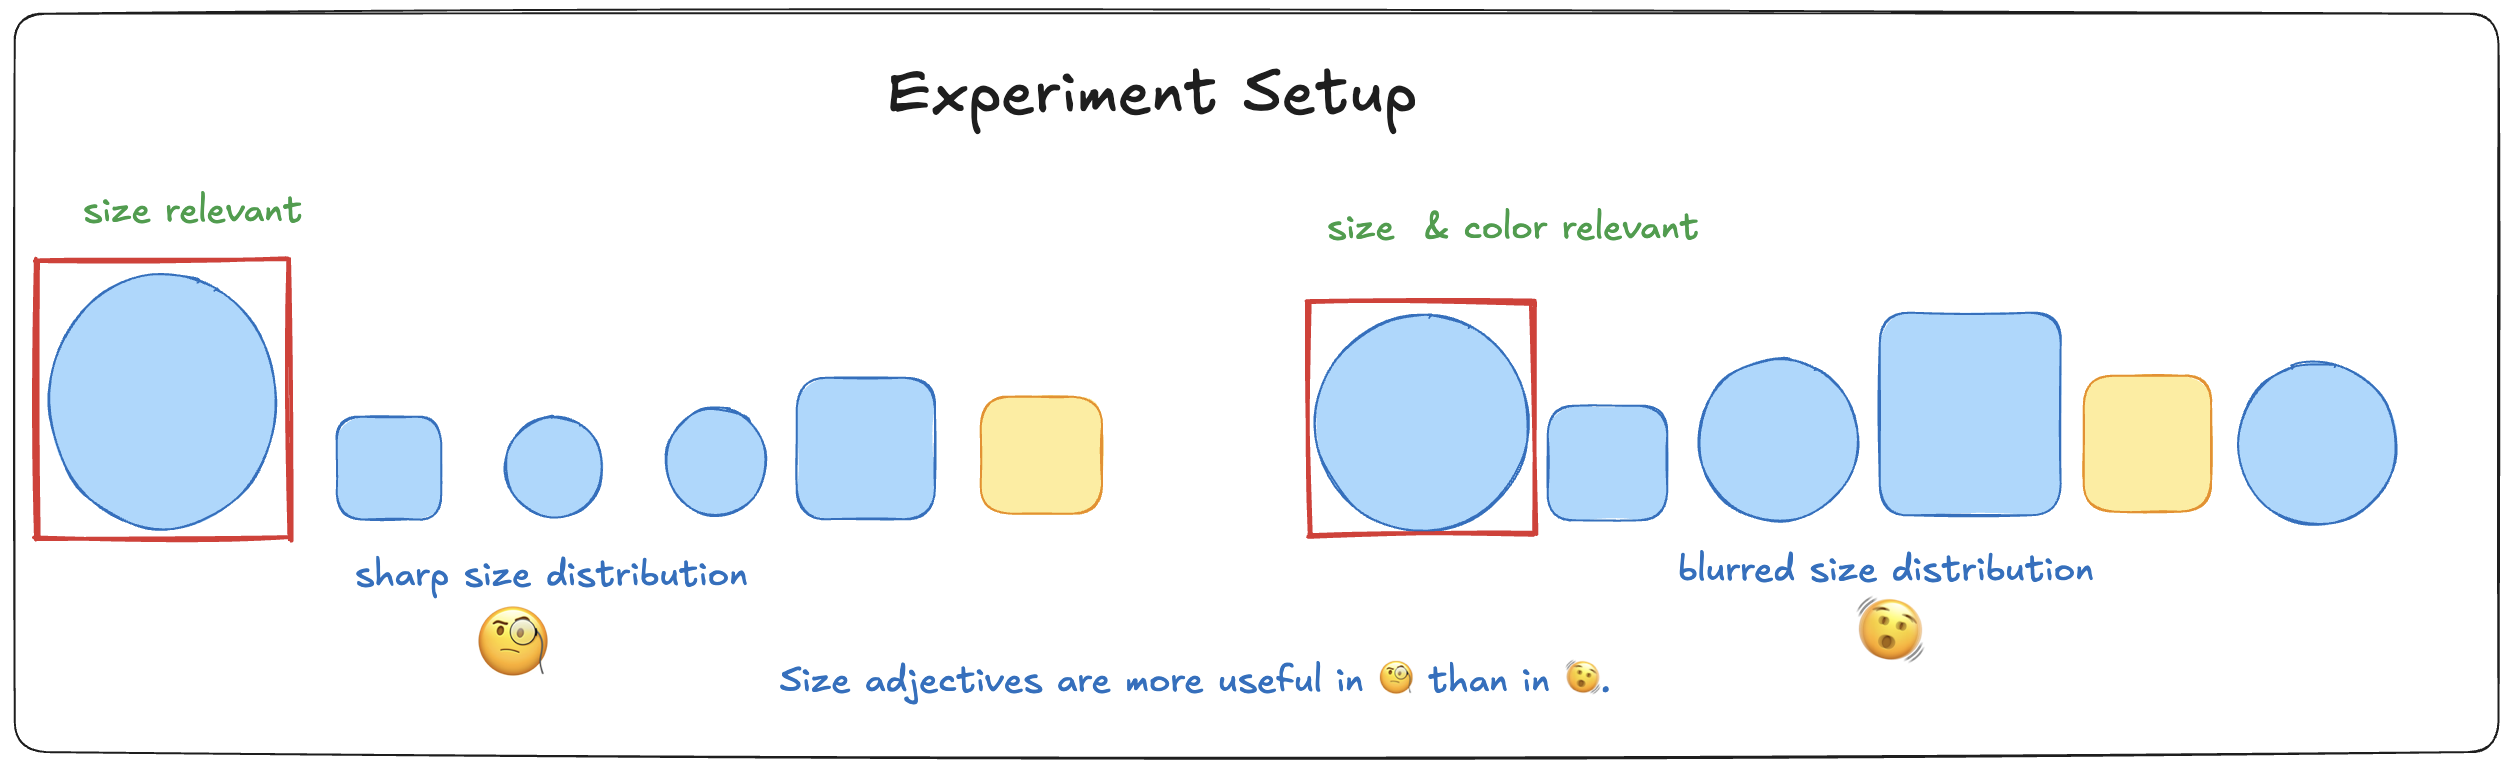
\includegraphics[width=0.72\textwidth]{experiment_item_illustration.png}
  \caption{Illustration of an experimental item. The referent (circled) is the largest, colour-matching, form-matching object in a six-object display. The two panels illustrate high- and low-discriminability size conditions.}
  \label{fig:item}
\end{figure}

\subsubsection{Procedure}

Participants completed the experiments online via Prolific and were instructed to identify the framed target using its perceptual properties, not spatial descriptions such as \emph{left} or \emph{right}.
The cover story framed each trial as a telephone conversation about collectible stickers: participants saw a set of six stickers on screen, one highlighted by a coloured frame, and were asked to refer to the target for a partner who could see the same stickers but neither the frame nor the spatial layout.
This made spatial terms uninformative and forced reliance on adjective descriptions.
Both experiments began with a consent form and a brief practice block (three training trials with feedback) that familiarised participants with the interface and the referential task.
The main trials were divided into four blocks of approximately equal length, with self-paced breaks between blocks.
Trial order within each block was randomised independently for each participant.
The two experiments differed in response format: Experiment~1 presented two competing adjective orders on a continuous slider (180 trials total, drawn from one of six counterbalanced lists), whereas Experiment~2 asked participants to type the adjective material they would place before the noun (135 trials, again from one of six lists, plus two additional dictionary-style practice items).
Despite this difference, both tasks probed the same question: whether adjective ordering tracks baseline size-first preferences, referential context, and the discriminatory value of size in the current display.

\subsection{Experiment 1: Slider-Rating Study}
\label{sec:exp:slider}

\subsubsection{Participants}

Participants ($N = 134$ after exclusions; 70 low discriminability, 64 high discriminability) were recruited online via Prolific and reported German as their native or fluent language.
Exclusion criteria were: more than three missing trial-list entries, completion times more than two standard deviations from the sample mean, more than three failures on control items, or more than three ``none fits'' responses on experimental items.
The analysed dataset contained 10{,}606 critical observations.
Mean completion time was 27.6 minutes.
Participants were compensated via Prolific at a rate above the platform-recommended minimum.

\subsubsection{Task and Scoring}

Experiment~1 implemented the shared referential design as a comparative judgment task.
Participants were asked to imagine a referential exchange about sticker collections and to evaluate which description would be better for identifying the framed target.
On each critical trial, two competing adjective orders appeared on opposite sides of a continuous slider, together with a ``none of the descriptions fits'' option.
Left--right presentation of the two orders was randomised across trials.
Each participant saw one of six lists built from the 27 underlying scenes, yielding 81 critical trials and 99 filler and control trials (180 total).
The filler and control items discouraged fixed response strategies and ensured attention to the referential task.
Raw slider values were recorded on a 0--100 scale and rescaled to $[-0.5, 0.5]$, with positive values indicating a size-first preference.
The descriptive analysis used a linear mixed-effects model with centred slider rating as the dependent variable and referential context, size discriminability, and their interaction as fixed effects, with random intercepts for participant and item.
For the Bayesian model comparison, these ratings were modelled with a Zero-One-Inflated Beta (ZOIB) likelihood to accommodate boundary mass at 0 and 1.

\subsubsection{Results}

\Cref{fig:slider-empirical} shows that size-first orderings were preferred across all three referential contexts, but the strength of the preference depended on which property was informative.
Referential context produced a large main effect, $F(2, 3349) = 213.7$, $p < .001$; $\chi^2(2) = 402.6$, $p < .001$.
The size-first preference was strongest in size-sufficient displays, intermediate in both-necessary displays, and weakest in colour-sufficient displays.
Notably, even colour-sufficient contexts did not produce a qualitative reversal: mean centred ratings remained above zero.

Size discriminability did not produce a reliable main effect, $F(1, 132) = 0.03$, $p = .86$, but it interacted with referential context, $F(2, 3349) = 5.84$, $p = .003$; $\chi^2(2) = 11.7$, $p = .003$.
The interaction was asymmetric: higher discriminability slightly increased the size-first preference in size-sufficient contexts (low: $0.30$, high: $0.34$) but slightly reduced it in both-necessary ($0.25$ vs.\ $0.20$) and colour-sufficient contexts ($0.06$ vs.\ $0.04$).
Post-hoc pairwise comparisons (Bonferroni-corrected) confirmed that no individual simple effect of discriminability within any referential context reached significance (all $p > .12$), indicating that the interaction is driven by the directional pattern across contexts rather than by any single cell contrast (see Appendix for full pairwise results).
This pattern is consistent with a discriminatory-strength interpretation: ordering preferences track the usefulness of size for identifying the target, but a baseline size-first tendency persists even when colour is locally more discriminating.
Specifically, P1--P3 predict exactly this profile: a size-first baseline persists across all contexts (P1), it weakens as colour becomes more discriminating (P2), and size discriminability matters only in interaction with referential context (P3).

\begin{figure}[htbp]
  \centering
  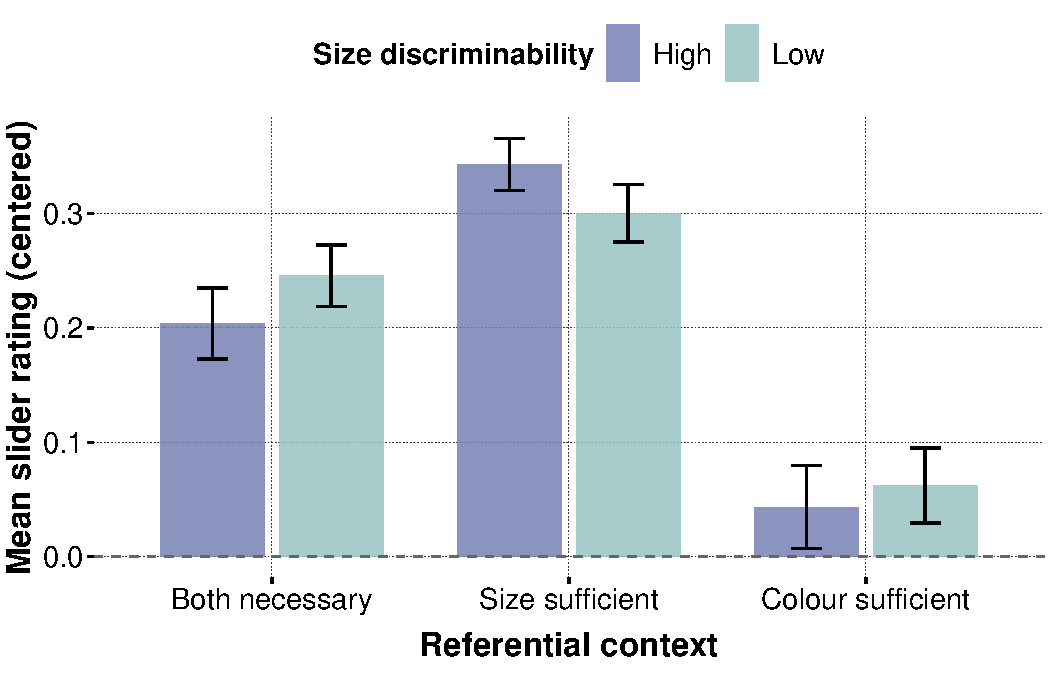
\includegraphics[width=0.88\textwidth]{slider_empirical.pdf}
  \caption{Empirical results from the slider-rating study. Mean centered slider ratings are shown by referential context and size discriminability, with 95\% confidence intervals. Positive values indicate a preference for size-first orderings.}
  \label{fig:slider-empirical}
\end{figure}

\subsection{Experiment 2: Free-Production Study}
\label{sec:exp:production}

\subsubsection{Participants}

Participants ($N = 113$ after exclusions; 60 low discriminability, 53 high discriminability) were recruited online via Prolific; anyone who had completed the slider study was excluded.
Further exclusion criteria were: completion times more than two standard deviations from the mean, more than 80\% identical responses, or more than 10\% missing or unannotatable responses.
The analysed dataset contained 9{,}639 critical observations.
Mean completion time was 32.4 minutes.
Compensation followed the same Prolific rate as Experiment~1.
\subsubsection{Task and Coding}

Experiment~2 used the shared referential design in a constrained production format.
Participants saw the framed target together with a sentence prompt and typed the adjective material needed before the noun \textit{Aufkleber}.
Restricting the response to the adjective slot rather than eliciting a full sentence reduced off-task variability and provided a controlled basis for coding.
Instructions again prohibited spatial descriptions, and a practice block familiarised participants with the relevant colour and form vocabulary before the critical trials began.
Each list contained 81 critical trials; the filler load was reduced relative to Experiment~1 (135 total trials vs.\ 180) to accommodate the greater time burden of typed production.

Responses were coded into 15 utterance categories corresponding to all one-, two-, and three-adjective strings built from size, colour, and form terms (3 one-adjective, 6 two-adjective, 6 three-adjective).
Misspellings and transparent lexical alternatives were normalised when their semantic class was unambiguous; spatial descriptions, comparative or ordinal size expressions, and other unclassifiable responses were excluded.
The dependent variable for the Bayesian model comparison is the categorical utterance label $y_i \in \{1, \ldots, 15\}$ for each trial $i$.
For descriptive statistics and targeted mixed-effects analyses, we also tracked two derived binary outcomes: whether an utterance was size-initial and whether it was over-informative (i.e., a three-adjective response in both-necessary contexts, or a multi-adjective response in size-sufficient or colour-sufficient contexts).

\subsubsection{Results}

The production data show stronger context sensitivity than the slider ratings.
As \Cref{fig:production-empirical} illustrates, size-first utterances dominated in size-sufficient contexts, colour-first utterances dominated in colour-sufficient contexts, and both-necessary contexts fell between the two extremes.
A mixed-effects logistic regression on size-initial responses yielded a strong main effect of referential context, $\chi^2(2) = 1859.7$, $p < .001$, no reliable main effect of size discriminability, $\chi^2(1) = 0.79$, $p = .37$, and a reliable interaction, $\chi^2(2) = 31.4$, $p < .001$.
As in the slider data, the interaction was asymmetric: higher discriminability reduced the size-first advantage in size-sufficient contexts but increased it in both-necessary contexts.

A complementary analysis of over-informativity reveals a related efficiency pressure.
Over-informative utterances were most frequent in size-sufficient contexts and least frequent in colour-sufficient contexts, producing a strong main effect of referential context, $\chi^2(2) = 725.7$, $p < .001$.
Unlike size-initiality, over-informativity also showed a main effect of size discriminability, $\chi^2(1) = 10.3$, $p = .001$, with more multi-adjective responses in low- than in high-discriminability displays.
This effect interacted with referential context, $\chi^2(2) = 63.8$, $p < .001$, driven primarily by size-sufficient contexts.
The pattern aligns with the broader communicative-efficiency literature on redundancy: speakers produce additional material when it helps resolve reference, even if it is not strictly necessary for uniqueness.
These results carry P1--P3 into unconstrained production --- with the size-first baseline (P1) attenuated where colour alone identifies the referent, even as the context modulation (P2) and the interaction-limited role of size discriminability (P3) emerge more sharply than in the slider task --- and additionally confirm P4: the richer response space reveals a graded over-informativity pattern that the binary slider task cannot show.

\begin{figure}[htbp]
  \centering
  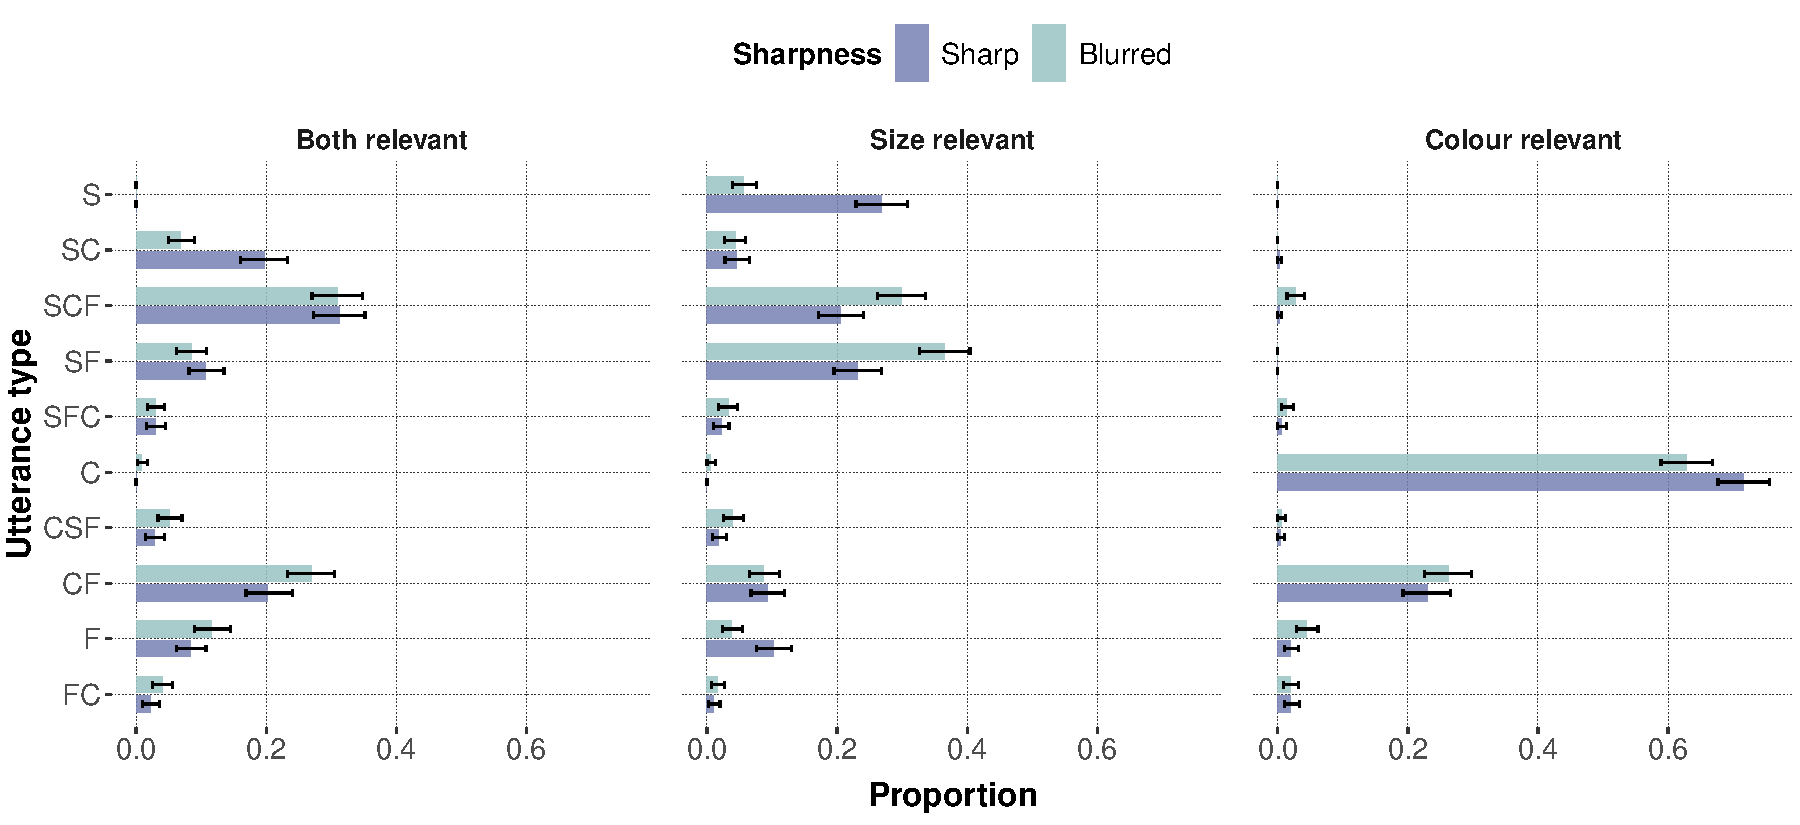
\includegraphics[width=0.95\textwidth]{production_empirical.pdf}
  \caption{Empirical results from the free-production study. Proportions of the major utterance types are shown by referential context and size discriminability, with bootstrapped 95\% confidence intervals. Only utterance types reaching at least 2\% in one condition are displayed.}
  \label{fig:production-empirical}
\end{figure}

\subsection{Interim Summary}

Across both experiments, three empirical regularities emerge.
First, there is a robust baseline preference for size-first orderings that persists even when colour is the only discriminating property.
Second, this preference is modulated by referential context: size-first choices increase when size is informative and decrease when colour is more useful, consistent with a discriminatory-efficiency account.
Third, size discriminability interacts with referential context but does not produce reliable main effects, suggesting that the sharpness of the size contrast acts as a secondary modulator rather than a primary driver.
The production data amplify these patterns relative to the slider data: free production elicits stronger context sensitivity and reveals a complementary over-informativity gradient driven by the same referential pressures.
Together, these results motivate a formal model that can capture both the stable ordering bias and its context-dependent modulation, while accommodating the richer response space of unconstrained production.

% =============================================================================
\section{Computational Model}
\label{sec:model}
% =============================================================================

This section formalizes the modelling framework introduced in \Cref{sec:framework}.
It specifies the literal-listener semantics, the global and incremental speakers, the context-fixed and context-updating regimes, and the inference setup for the $2 \times 2$ model comparison.
The experiments were broader than the fitted model comparison: the full paradigm included size--form and colour--form trials, but the analyses reported here focus on size--colour scenes, where the theoretical contrast between a gradable adjective and a determinate feature adjective is clearest.
Form therefore remains part of the general representational vocabulary and of the production response space, but it is not the primary mechanistic contrast in the current fit.

\subsection{Representational Primitives}
\label{sec:model:primitives}

An object is a triple $o = (s, c, f)$, where $s \in [1,10]$ denotes size, $c \in \{0,1\}$ indicates colour match, and $f \in \{0,1\}$ indicates form match.
A context $\mathcal{C}$ is a set of $n_\text{obj}$ objects.
In the experiments, the intended referent is always the largest object with $c = f = 1$.

Utterances are built from three adjective types, \adj{S}, \adj{C}, and \adj{F}.
An utterance $u = (a_1, \ldots, a_T)$ is an ordered sequence of adjectives $a_t \in \{\adj{S}, \adj{C}, \adj{F}\}$ with $T \in \{1,2,3\}$.
Combining all lengths and orderings yields 15 surface forms:
\{\utter{S}, \utter{SC}, \utter{SCF}, \utter{SF}, \utter{SFC}, \utter{C}, \utter{CS}, \utter{CSF}, \utter{CF}, \utter{CFS}, \utter{F}, \utter{FS}, \utter{FSC}, \utter{FC}, \utter{FCS}\}.
This full inventory reflects the broader experimental vocabulary.
For the reported model fits, however, the scene subset is size--colour: \adj{C} denotes the determinate feature that competes with size for identification, while \adj{F} remains available chiefly as an additional, potentially redundant modifier in production.

\subsection{Meaning Functions}
\label{sec:model:semantics}

\paragraph{Context-dependent size semantics.}
We model size adjectives with a context-sensitive threshold semantics following \citet{schmidt2009how}, who showed that the interpretation of gradable adjectives depends on the statistics of the comparison class.
\citet{franke2019subjectivity} adopted the same approach in their simulation of adjective-ordering preferences.
A threshold is computed from the current comparison class $\mathcal{C}$:
\begin{equation}
  \theta_k(\mathcal{C})
  = x_\text{max}(\mathcal{C})
    - k \,\bigl(x_\text{max}(\mathcal{C}) - x_\text{min}(\mathcal{C})\bigr),
  \label{eq:threshold}
\end{equation}
where $x_\text{min}(\mathcal{C})$ and $x_\text{max}(\mathcal{C})$ are the lower and upper bounds of the mid-range of the contextual size distribution and $k \in [0,1]$ controls how permissively ``big'' is applied.
The resulting semantic value $\llbracket\text{S}\rrbracket(o, \mathcal{C}) \in [0,1]$ is graded rather than binary: an object's size is compared to the threshold via a normal slack function scaled by a perceptual-blur parameter $w_f$, consistent with scalar variability in the Approximate Number System \citep{feigenson2004core}.
This context dependence is what makes the context-fixed vs.\ context-updating distinction possible: because $\theta_k$ depends on $\mathcal{C}$, changing which objects are in the comparison class changes what counts as big.

\paragraph{Colour and form semantics.}
Colour and form are in principle determinate: an object either matches the feature or it does not.
Following the relaxed-semantics approach of \citet{degen2020redundancy} and \citet{waldon2021modeling}, however, we soften these denotations by parameterizing them with $\nu \in (0,1)$, which can be interpreted as the probability that a feature-matching object is correctly described by the adjective.
This relaxation allows even determinate properties to carry graded information, which is important for modeling redundant modification.
In the reported model fits, colour is the primary determinate comparison case because inference is carried out on size--colour scenes, whereas form is retained as a general determinate feature term and as a possible redundant modifier in production.
In the slider models, colour and form share a single $\nu$ parameter.
In the production models, they receive separate fixed values, $\nu_\text{colour}$ and $\nu_\text{form}$, obtained from a preliminary inference run and held constant across all model variants.

\subsection{Incremental Listener}
\label{sec:model:composition}

The literal listener constructs utterance meanings incrementally by combining token-level semantic contributions while updating the effective comparison class.
Let $u = (w_1, \ldots, w_T)$ be an utterance.
The listener maintains a sequence of belief states $\{P_t(o)\}_{t=0}^{T}$, where $P_t(o)$ denotes the posterior belief after incorporating the suffix $(w_{t+1}, \ldots, w_T)$:
\begin{equation}
  P_t(o) = P\bigl(o \mid w_{t+1}, \ldots, w_T\bigr), \qquad t = 0, \ldots, T,
  \label{eq:listener_belief}
\end{equation}
with base case
\begin{equation}
  P_T(o) = P_{\mathrm{prior}}(o).
  \label{eq:listener_base}
\end{equation}
For $t = T, T-1, \ldots, 1$, beliefs are updated according to
\begin{equation}
  P_{t-1}(o) \propto P_t(o)\,\llbracket w_t \rrbracket(o),
  \label{eq:comp}
\end{equation}
which normalizes to
\begin{equation}
  P_{t-1}(o) = \frac{P_t(o)\,\llbracket w_t \rrbracket(o)}{\sum_{o'} P_t(o')\,\llbracket w_t \rrbracket(o')}.
  \label{eq:comp_norm}
\end{equation}
After all tokens have been processed, the listener arrives at
\begin{equation}
  P_0(o) = P(o \mid u).
  \label{eq:listener_final}
\end{equation}

The composition rule in \Cref{eq:comp} is shared by both semantic regimes of the model.
What differs is how the meaning function $\llbracket w_t \rrbracket$ is computed for gradable adjectives such as size.

\paragraph{Context-updating semantics.}
Under the context-updating regime, the size threshold $\theta_k$ is recomputed from the listener's current belief state at each composition step:
\begin{equation}
  \llbracket w_t \rrbracket_{\textsc{upd}}(o)
  \;=\; \llbracket w_t \rrbracket_{P_t}(o),
  \label{eq:context_updating}
\end{equation}
where $P_t$ is the posterior after processing all words to the right of position $t$.
The current belief state therefore plays a dual role: it serves as the prior for the next update step, and it determines the semantics of the next token.
Because $P_t$ itself depends on the semantics of later words, this creates a feedback loop:
\begin{equation}
  \llbracket w_t \rrbracket_{P_t}
  \quad\text{depends on}\quad
  P_t(o) \propto P_{t+1}(o)\,\llbracket w_{t+1} \rrbracket_{P_{t+1}}(o).
  \label{eq:context_recursion}
\end{equation}
Word order changes the sequence of comparison classes and thereby the interpretation of the utterance, yielding non-commutativity:
\begin{equation}
  P(o \mid w_1, w_2) \neq P(o \mid w_2, w_1)
  \quad\text{in general.}
  \label{eq:noncommutativity}
\end{equation}

\paragraph{Context-fixed semantics.}
Under the context-fixed regime, the size threshold is computed once from the scene prior and held constant throughout composition:
\begin{equation}
  \llbracket w_t \rrbracket_{\textsc{fix}}(o)
  \;=\; \llbracket w_t \rrbracket_{P_{\mathrm{prior}}}(o)
  \quad\text{for all } t.
  \label{eq:context_fixed}
\end{equation}
The listener's beliefs still update incrementally via \Cref{eq:comp}, but this update no longer feeds back into the meaning function.
For deterministic adjectives such as colour and form, both regimes are identical because their semantics does not depend on the comparison class.
The context-fixed regime therefore isolates the contribution of incremental belief updating from the additional effect of posterior-dependent meaning.

\subsection{Utterance Prior and Speaker Models}
\label{sec:model:speakers}

The model incorporates a prior over utterance forms that is separate from the pragmatic component.
This prior captures stable ordering tendencies --- such as the well-documented subjectivity-driven size-first preference --- that the speaker brings to the task before any scene-specific pragmatic reasoning.

In the slider-rating models, the prior is minimal: a single inferred bias parameter $b \geq 0$ that penalizes the reverse (colour-first) order relative to the canonical (size-first) order.
Because $b$ is estimated from data rather than fixed, the posterior indicates how much residual ordering preference remains after the RSA mechanism has been applied; if the pragmatic model were sufficient on its own, the posterior for $b$ would concentrate near zero.

In the production models, the prior is richer: a language-model distribution $P_\text{LM}(u)$ over the 15 utterance forms, derived from German GPT-2 surprisal estimates averaged across the experimental adjective--noun combinations.
The contribution of this prior is scaled by an inferred parameter $\beta$, yielding utterance cost $\text{cost}_\text{LM}(u) = -\beta \log P_\text{LM}(u)$.
Like $b$ in the slider model, the LM prior encodes stable word-order tendencies from language experience, which the pragmatic speaker then modulates in light of the current scene.

\paragraph{Global speaker.}
The global speaker computes a distribution over complete utterances by applying a softmax to utterance-level utility:
\begin{equation}
  S_{\text{gb}}(u \mid o)
  = \frac{\exp\!\bigl(U(o,u)\bigr)}{\sum_{u'} \exp\!\bigl(U(o,u')\bigr)}.
  \label{eq:global_speaker}
\end{equation}
For the production model, utility is defined as
\begin{equation}
  U(o^\ast,u)
  = \alpha\,\log L(o^\ast \mid u) + \beta\,\log P_{\mathrm{LM}}(u),
  \label{eq:global_utility}
\end{equation}
where $\alpha$ is the RSA rationality parameter.
In the slider-rating models, the utility simplifies to
\begin{equation}
  U(o,u) = \alpha\bigl(\log L(o \mid u) - b_u\bigr),
  \label{eq:slider_utility}
\end{equation}
where $b_u = 0$ for the size-first order and $b_u = b$ for the reverse order.

\paragraph{Incremental speaker.}
The incremental speaker chooses one token at a time. For an intended referent $o^\ast$,
\begin{equation}
  S_{\mathrm{inc}}(u \mid o^\ast)
  = \prod_{t=1}^{T} S_t\!\left(w_t \mid u_{<t}, o^\ast\right),
  \qquad u_{<t} = (w_1, \ldots, w_{t-1}),
  \label{eq:inc_chain}
\end{equation}
with local decision rule
\begin{equation}
  S_t(a \mid u_{<t}, o^\ast)
  \propto
  \bigl[L(o^\ast \mid u_{<t} + a)\bigr]^{\alpha}.
  \label{eq:inc_speaker}
\end{equation}
Combining local pragmatic choice with utterance-level cost yields, for the production model,
\begin{equation}
  S_{\mathrm{inc}}(u \mid o^\ast)
  \propto P_{\mathrm{LM}}(u)^{\beta}
  \cdot \prod_{t=1}^{T}
  \frac{\bigl[L(o^\ast \mid u_{<t} + w_t)\bigr]^{\alpha}}{Z_t(u_{<t}, o^\ast)},
  \label{eq:inc_full}
\end{equation}
where
\begin{equation}
  Z_t(u_{<t}, o^\ast)
  = \sum_{a} \bigl[L(o^\ast \mid u_{<t} + a)\bigr]^{\alpha}
  \label{eq:inc_normaliser}
\end{equation}
ensures local normalization.
In the slider-rating models, the LM prior is replaced by the bias term: $S_{\mathrm{inc}}(u \mid o^\ast) \propto \exp(-b_u) \cdot \prod_t S_t(w_t \mid u_{<t}, o^\ast)$.
The theoretical contrast is that the global speaker applies pragmatic reasoning once over complete utterances, whereas the incremental speaker applies it at each token position.
When semantics is context-dependent, these two model variants are not equivalent.

\subsection{Model Variants and Inference}
\label{sec:model:variants}

We report a $2 \times 2$ model comparison that crosses two theoretically motivated dimensions: \emph{speaker architecture} (global vs.\ incremental) and \emph{semantic regime} (context-fixed vs.\ context-updating).
All four variants use hierarchical participant pooling, which consistently outperforms pooled alternatives (see Appendix).
The speaker-architecture contrast asks whether word-by-word production planning adds explanatory value beyond utterance-level evaluation.
The semantic-regime contrast asks whether recomputing the size threshold from the listener's evolving belief state adds value beyond a fixed comparison class.
Their interaction tests whether these two mechanisms are synergistic.

The two semantic regimes --- context-updating (\Cref{eq:context_updating}) and context-fixed (\Cref{eq:context_fixed}) --- are defined formally above.
All other aspects of the model, including the belief-update structure and the speaker's decision rule, remain identical across regimes.
The context-fixed variant therefore serves as a targeted ablation of the context-updating mechanism.

For the slider-rating models, the semantic parameters $k = 0.5$, $w_f = 1.0$, and a single shared feature reliability $\nu = 0.85$ (colour and form) are fixed across all variants.
Their influence on model predictions is explored in the simulation study below.
The free-production comparison is run on an extended speaker model whose fixed constants are calibrated empirically; this extension and its calibration are developed in \Cref{sec:model:extended}.

\begin{table}[htbp]
  \caption{Slider-rating model variants ($2 \times 2$: speaker $\times$ semantics, all hierarchical)}
  \label{tab:slider-models}
  \centering
  \begin{tabularx}{\textwidth}{llXl}
    \toprule
    \textbf{Model} & \textbf{Speaker} & \textbf{Size semantics} & \textbf{Inferred parameters} \\
    \midrule
    Global, context-fixed & $S_\text{G}$ & Fixed threshold from scene prior & $\alpha,\; b,\; \sigma,\; \tau,\; \delta_i$ \\
    Global, context-updating & $S_\text{G}$ & Threshold updated from listener posterior & $\alpha,\; b,\; \sigma,\; \tau,\; \delta_i$ \\
    Incremental, context-fixed & $S_\text{I}$ & Fixed threshold from scene prior & $\alpha,\; b,\; \sigma,\; \tau,\; \delta_i$ \\
    Incremental, context-updating & $S_\text{I}$ & Threshold updated from listener posterior & $\alpha,\; b,\; \sigma,\; \tau,\; \delta_i$ \\
    \bottomrule
  \end{tabularx}
\end{table}

\begin{table}[htbp]
  \caption{Free-production model variants ($2 \times 2$: speaker $\times$ semantics, all hierarchical).
  The four cells are instantiated on the extended production model of \Cref{sec:model:extended} and are \emph{parameter-matched}: every cell carries the identical nominal inventory (the ten population parameters of \Cref{tab:param-inventory} plus the 339-element participant hierarchy and the five calibrated constants).
  Context-fixed is the nested restriction of context-updating obtained by freezing the listener's threshold, and global vs.\ incremental is a structural switch with no extra parameters, so any fit difference is structural rather than a complexity artifact.}
  \label{tab:production-models}
  \centering
  \begin{tabularx}{\textwidth}{llXl}
    \toprule
    \textbf{Model} & \textbf{Speaker} & \textbf{Size semantics} & \textbf{Nominal inventory} \\
    \midrule
    Global, context-fixed & $S_\text{G}$ & Fixed threshold from scene prior & 10 population $+\;\delta_i$ \\
    Global, context-updating & $S_\text{G}$ & Threshold updated from listener posterior & 10 population $+\;\delta_i$ \\
    Incremental, context-fixed & $S_\text{I}$ & Fixed threshold from scene prior & 10 population $+\;\delta_i$ \\
    Incremental, context-updating & $S_\text{I}$ & Threshold updated from listener posterior & 10 population $+\;\delta_i$ \\
    \bottomrule
  \end{tabularx}
\end{table}

All models were implemented in NumPyro \citep{phan2019composable} and estimated with the NUTS sampler \citep{hoffman2014no}.
Convergence was assessed via split-$\hat{R}$, effective sample size, divergence counts, and posterior predictive checks.

The two datasets required different likelihood specifications.
Slider responses showed substantial mass at the boundaries (0 and 1), which motivated a Zero-One-Inflated Beta (ZOIB) likelihood rather than a Gaussian approximation.
The free-production data were categorical and highly skewed, with many utterance types near zero frequency in some conditions.
To keep inference stable and the comparison interpretable, the semantic constants were fixed at common values across all variants and only the pragmatic parameters were estimated from data.
This ensures that any difference in fit between variants reflects the speaker architecture and semantic regime, not incidental variation in lexical semantics.
The next subsection develops the extended production speaker and the principled procedure by which its parameter set and fixed constants were selected.

\subsection{An Extended Production Model}
\label{sec:model:extended}

The slider task contrasts only two competing orders, and there a minimal speaker --- a single rationality parameter $\alpha$, the language-model weight $\beta$, and a participant-level offset --- already reproduces the condition-level pattern almost perfectly (\Cref{sec:modelcomparison}).
Free production is a fifteen-way choice over the full inventory of one-, two-, and three-adjective strings, and a process account we are willing to advocate for that setting should fit it well with a parameter set that is motivated and selected by an explicit criterion rather than hand-tuned to residuals.
We therefore develop the production speaker by extending the incremental speaker with a small number of independently motivated components and then pruning them with a parsimony frontier and a fixed-constant sensitivity analysis.

\paragraph{Additional components.}
Each component targets a documented property of production or of the adjective-ordering literature, not a particular residual cell.
\emph{Per-dimension rationality} replaces the single $\alpha$ with separate informativity weights for size and colour ($\alpha_\text{S}$, $\alpha_\text{C}$), since the two adjective types differ in how reliably they discriminate.
A \emph{canonical-order penalty} ($\lambda_\text{noncanon}$) discounts utterances that place form before colour, encoding the cross-linguistically robust colour-before-form tendency \citep{sproat1991cross, cinque1994, scott2002}.
A \emph{sufficiency boost} ($\lambda_\text{suff}$) raises the probability of beginning with the single dimension that already singles out the referent.
A \emph{context-gated form-mention boost} ($\lambda_\text{form-mod}$) captures the additional, often redundant mention of form when neither size nor colour alone resolves the scene.
A \emph{graded length bias} ($\gamma_\text{base}$, $\gamma_\text{one}$, $\gamma_\text{sharp}$) modulates the tendency to produce longer or shorter descriptions, including extra modification when the size cue is perceptually blurred.
A \emph{lapse rate} ($\epsilon$) mixes the speaker distribution with a uniform component, absorbing inattentive responses instead of distorting the pragmatic parameters.
Finally, the determinate feature semantics are \emph{softened and anchored}: colour and form are given graded denotations (as in the slider model) with empirically calibrated reliabilities rather than treated as deterministic.

\paragraph{A parsimony frontier.}
We did not choose this component set by hand.
We fitted the maximal model (thirteen population parameters plus the participant hierarchy) and then walked a leave-one-out frontier, removing one coefficient at a time and refitting (\Cref{tab:parsimony-frontier}).
Three coefficients carry no fit information and were dropped at zero cost, each for an independent reason: the language-model temperature pins to a stable value and can be fixed without reallocating the canonical-order signal; an erdc-gated three-word penalty collapsed onto zero in the joint posterior; and the form informativity weight $\alpha_\text{F}$ had a posterior interval spanning zero, because form is already produced through the language-model prior, the anchored semantics, and the form-mention boost.
Removing all three yields a ten-parameter model that is statistically indistinguishable from the maximal model, with every retained coefficient's $94\%$ HDI excluding zero.
This is the frontier floor: dropping either $\lambda_\text{suff}$ or $\gamma_\text{sharp}$ beyond this point costs measurable fit, so the remaining ten coefficients are load-bearing.
We report this ten-parameter model, with the maximal model and the frontier as the selection evidence.

\begin{table}[htbp]
\centering
\caption{Parsimony frontier for the extended production speaker (size--colour subset, four chains, hierarchical).
$R^2_{\text{all}}$ uses all condition $\times$ utterance cells; $R^2_{\ge.02}$ restricts to behaviourally relevant cells (empirical proportion $\ge 0.02$); $r$ is the Pearson correlation between predicted and observed proportions.
The first three rows remove coefficients at zero fit cost; the last two show the frontier floor, where further removal costs fit.}
\label{tab:parsimony-frontier}
\small
\begin{tabular}{lrrrr}
\hline
Model & \#named & $R^2_{\text{all}}$ & $R^2_{\ge.02}$ & $r$ \\
\hline
Maximal model & 13 & $0.919$ & $0.919$ & $0.959$ \\
\quad $-$ LM temperature & 12 & $0.920$ & $0.919$ & $0.959$ \\
\quad $-$ LM temp.\ $-$ 3-word penalty & 11 & $0.920$ & $0.920$ & $0.959$ \\
\quad $-$ also $\alpha_\text{F}$ \textbf{(reported)} & \textbf{10} & $\mathbf{0.921}$ & $\mathbf{0.921}$ & $\mathbf{0.959}$ \\
\quad\quad $-$ also $\lambda_\text{suff}$ & 10 & $0.909$ & $0.904$ & $0.954$ \\
\quad\quad $-$ also $\gamma_\text{sharp}$ & 10 & $0.900$ & $0.889$ & $0.949$ \\
\hline
\end{tabular}
\end{table}

\paragraph{Calibrating the fixed semantic constants.}
The ten-parameter model still depends on four constants held fixed during inference: the colour reliability $\nu_\text{colour}$, the form reliability $\nu_\text{form}$, the size-threshold anchor $k$, and the size-sigmoid sharpness $w_f$.
We audited all four (\Cref{tab:semval-refit}).
A cheap static sweep --- varying one constant while holding the ten fitted parameters at their values --- suggested that the originally assumed near-deterministic colour reliability ($\nu_\text{colour}=0.97$) was near-optimal.
A joint refit that lets the colour weight readjust tells the opposite story: freeing $\nu_\text{colour}$ moves it to $0.59$ $[0.56, 0.62]$ and gains $+0.022$ $R^2$.
The static sweep is misleading here because the constant trades off against the fitted parameters; only a joint refit licenses a conclusion about a fixed constant.
Re-fixing $\nu_\text{colour}$ at the freed posterior mean ($0.59$) recovers the entire gain at ten parameters with clean sampling, dominating both the original value and freeing the constant.
The other three constants are kept fixed: freeing each alone gains essentially nothing, the form reliability is unidentified, the sharpness brackets its fixed value, and freeing all four jointly produces a non-identified ridge (effective sample sizes in the single digits), a caution against over-parameterising the semantics.

The soft colour predicate also has a theoretical reading.
Moving $\nu_\text{colour}$ from $0.97$ to $0.59$ roughly tripled the colour informativity weight ($\alpha_\text{C}$: $1.3 \to 3.8$), raised the size weight ($\alpha_\text{S}$: $6.2 \to 8.0$), strengthened the canonical-order penalty, and roughly halved the lapse rate ($\epsilon$: $0.18 \to 0.11$).
A near-deterministic colour denotation suppresses the pragmatic weight on colour and dumps the resulting misfit into uniform noise; softening it to a roughly $60\%$-reliable predicate lets the informativity weights be estimated properly and lets far less of the data be explained away as inattention.
The data prefer a colour adjective that is graded rather than categorical, consistent with the relaxed-semantics motivation for $\nu$ and sharper than the near-deterministic value originally assumed.

\begin{table}[htbp]
\centering
\caption{Fixed-constant sensitivity analysis for the ten-parameter production model (joint refits, size--colour subset).
Each ``free'' row frees one constant and refits all parameters jointly; ``free all four'' frees them together.
$\Delta R^2$ is relative to the reported model.
Only $\nu_\text{colour}$ warrants a changed value; it is re-fixed at its freed posterior mean.}
\label{tab:semval-refit}
\small
\begin{tabular}{lrrl}
\hline
Refit & \#named & $R^2_{\text{all}}$ & Freed posterior / verdict \\
\hline
Reported ($\nu_\text{colour}=0.97$, all fixed) & 10 & $0.921$ & --- \\
Free $\nu_\text{colour}$ & 11 & $0.942$ & $0.59\;[0.56,0.62]$; large gain \\
Free $\nu_\text{form}$ & 11 & $0.920$ & unidentified (HDI spans prior) \\
Free $k$ & 11 & $0.921$ & negligible gain \\
Free $w_f$ & 11 & $0.921$ & brackets fixed value \\
Free all four & 14 & $0.953$ & non-identified ridge (ESS 6--28) \\
\textbf{$\nu_\text{colour}$ re-fixed at $0.59$ (reported)} & \textbf{10} & $\mathbf{0.942}$ & clean sampling, $r = 0.97$ \\
\hline
\end{tabular}
\end{table}

The resulting model --- ten population parameters, the participant hierarchy, and five empirically calibrated constants ($\nu_\text{colour}=0.59$, $\nu_\text{form}=0.50$, $k=0.50$, $w_f=0.69$, and the fixed LM temperature) --- explains $R^2 \approx 0.94$ of the cell-level production variance ($r = 0.97$).
This is the model we advocate for production, and the architecture on which the $2 \times 2$ comparison below is instantiated.
Its full parameter inventory and priors are given in \Cref{tab:param-inventory}.

% =============================================================================
\section{Bayesian Model Comparison}
\label{sec:modelcomparison}
% =============================================================================

We evaluated the four model variants (\Cref{tab:slider-models,tab:production-models}) against both datasets using Pareto-smoothed importance-sampling leave-one-out cross-validation \citep[PSIS-LOO;][]{vehtari2017practical}.
All models were estimated with four MCMC chains using the No-U-Turn Sampler \citep[NUTS;][]{hoffman2014no} as implemented in NumPyro \citep{phan2019composable}.
For the slider models, each chain drew 500 warmup and 500 post-warmup samples (target acceptance probability $= 0.90$, maximum tree depth $= 8$).
For the production models, each chain drew 5{,}000 warmup and 2{,}000 post-warmup samples (target acceptance probability $= 0.85$, maximum tree depth $= 7$).
Convergence was confirmed via split-$\hat{R} < 1.01$ and effective sample sizes exceeding 400 for all parameters across all models.
PSIS-LOO comparisons are reported as the difference in expected log pointwise predictive density ($\Delta$ELPD) relative to the best-fitting model, together with the difference standard error (dse).
A ratio $|\Delta\text{ELPD}|/\text{dse}$ substantially greater than 1 indicates a significant difference in out-of-sample predictive accuracy.
\Cref{tab:loo-summary} provides the full PSIS-LOO comparison for all eight models.

\begin{table}[htbp]
\centering
\caption{PSIS-LOO comparison for all models.
ELPD$_{\text{LOO}}$ is the absolute expected log pointwise predictive density; $\Delta$ELPD and dse are the difference and its standard error relative to the best-fitting model in each dataset; $p_{\text{LOO}}$ is the effective number of parameters.}
\label{tab:loo-summary}
\small
\begin{tabular}{llrrrr}
\hline
Dataset & Model & ELPD$_{\text{LOO}}$ & $\Delta$ELPD & dse & $p_{\text{LOO}}$ \\
\hline
\multicolumn{6}{l}{\textit{Slider-Rating Study}} \\
 & Incremental, context-updating & $-2{,}774.1$ & $0.0$ & --- & 64.8 \\
 & Incremental, context-fixed & $-2{,}774.1$ & $-0.1$ & $0.2$ & 65.1 \\
 & Global, context-updating & $-4{,}249.2$ & $-1{,}475.1$ & $65.9$ & 1{,}425.0 \\
 & Global, context-fixed & $-7{,}562.2$ & $-4{,}788.1$ & $127.2$ & 4{,}372.0 \\[4pt]
\multicolumn{6}{l}{\textit{Free-Production Study (extended model, parameter-matched)}} \\
 & Incremental, context-updating & $-5{,}275.0$ & $0.0$ & --- & 174.5 \\
 & Incremental, context-fixed & $-5{,}338.0$ & $-63.0$ & $14.0$ & 146.3 \\
 & Global, context-fixed & $-6{,}200.5$ & $-925.5$ & --- & 6.8 \\
 & Global, context-updating & $-6{,}207.6$ & $-932.6$ & --- & 6.6 \\
\hline
\end{tabular}
\end{table}

\subsection{Slider-Rating Study}

\Cref{fig:slider-model} shows the $2 \times 2$ comparison for the slider data.
The dominant contrast is speaker architecture: both incremental models fit the data well and are statistically indistinguishable ($\Delta\text{ELPD} = -0.1$, dse $= 0.2$), whereas both global models perform far worse ($\Delta\text{ELPD} > 1{,}400$).
Within the incremental pair, context-updating semantics confers no detectable advantage over context-fixed semantics.
For graded preference judgments between two competing orders, word-by-word pragmatic reasoning is therefore the dominant mechanism: it provides strong order sensitivity regardless of whether the size threshold is recomputed from the running posterior.
Posterior-predictive checks confirm that the incremental context-updating model captures the condition-level pattern well (\Cref{fig:slider-results}).
For the best-fitting incremental context-updating model, the posterior rationality parameter was $\alpha = 0.69$ ($\mathit{SD} = 0.06$, 94\% HDI $[0.57, 0.79]$), the ZOIB dispersion was $\sigma = 0.72$ ($\mathit{SD} = 0.01$, 94\% HDI $[0.70, 0.74]$), and the hierarchical spread of participant-level rationality offsets was $\tau = 0.12$ ($\mathit{SD} = 0.01$, 94\% HDI $[0.10, 0.14]$).
Crucially, the bias intercept was $b = 0.58$ ($\mathit{SD} = 0.06$, 94\% HDI $[0.47, 0.69]$), reliably above 0.50.
This positive bias means that even after the RSA mechanism accounts for context-dependent informativeness, the model infers a residual size-first preference --- consistent with the view that a stable ordering default persists beyond what discriminatory utility alone explains.
Within the global pair, context-updating semantics substantially outperforms context-fixed semantics ($\Delta\text{ELPD} \approx 3{,}313$, $|\Delta\text{ELPD}|/\text{dse} > 24$).
Context-updating composition thus provides a minimal source of order sensitivity that partially compensates for the lack of incrementality, but both global models remain far worse than either incremental variant.

\begin{figure}[htbp]
  \centering
  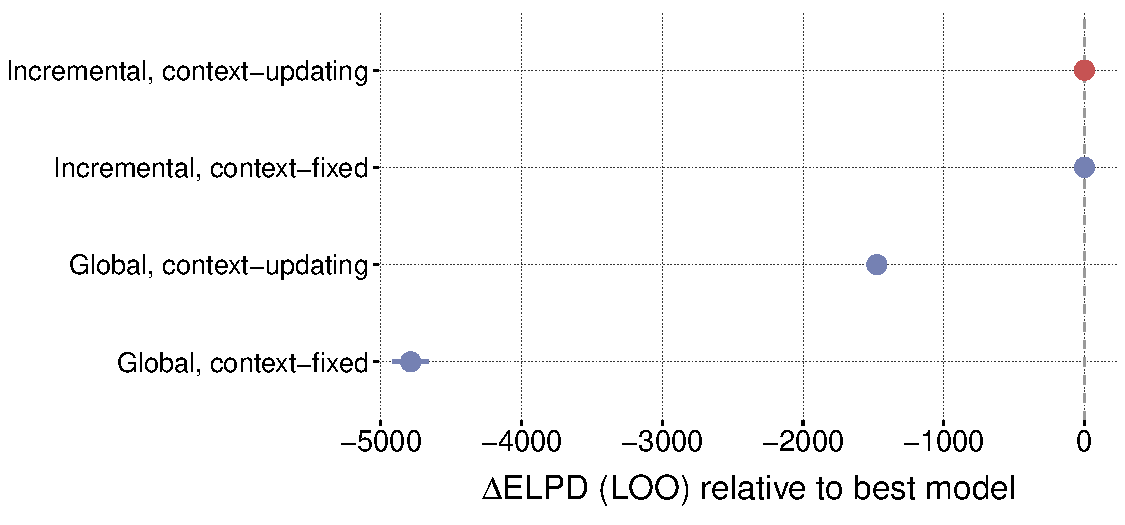
\includegraphics[width=0.65\textwidth]{slider_model_comparison.pdf}
  \caption{Slider-rating model comparison ($2 \times 2$: speaker $\times$ semantics). $\Delta$ELPD relative to the best model, with $\pm 1$ difference standard error. Models whose intervals exclude zero show significantly worse predictive performance.}
  \label{fig:slider-model}
\end{figure}

\begin{figure}[htbp]
  \centering
  \begin{minipage}[c]{0.52\textwidth}
    \centering
    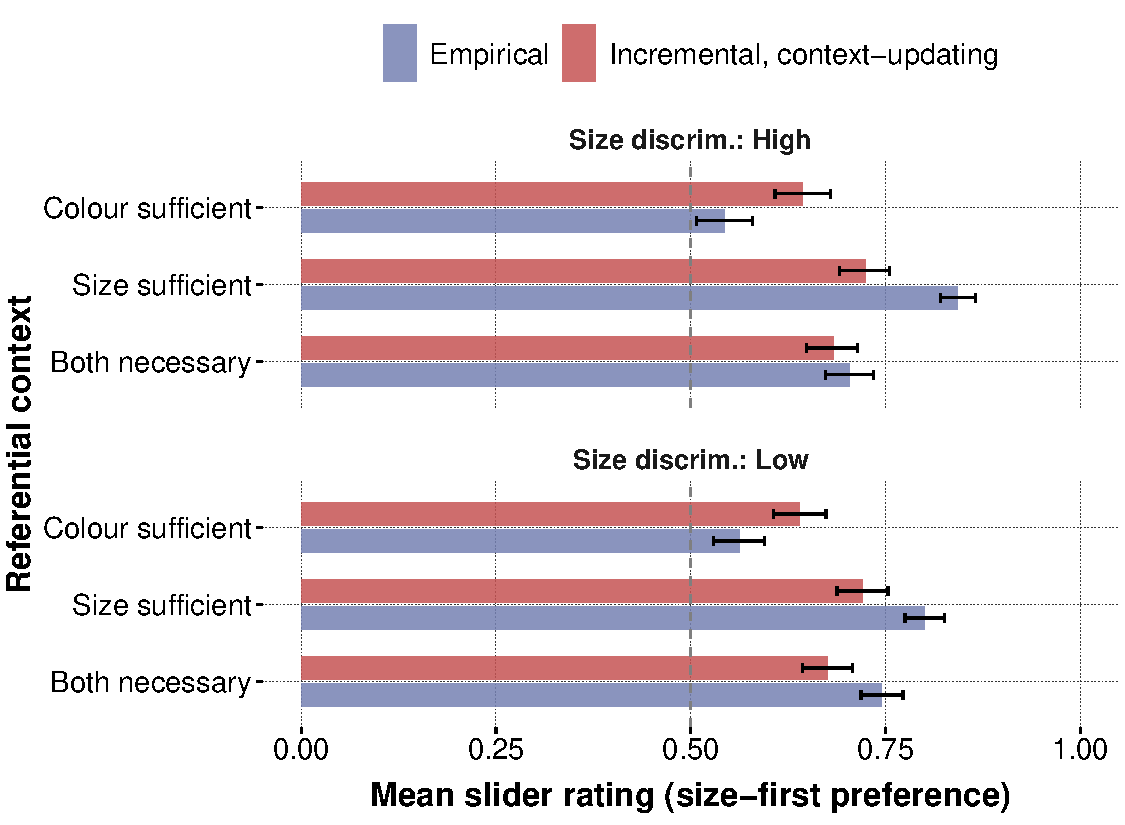
\includegraphics[width=\linewidth]{slider_ppc_best.pdf}\\[2pt]
    {\small (a) Mean rating by condition}
  \end{minipage}\hfill
  \begin{minipage}[c]{0.46\textwidth}
    \centering
    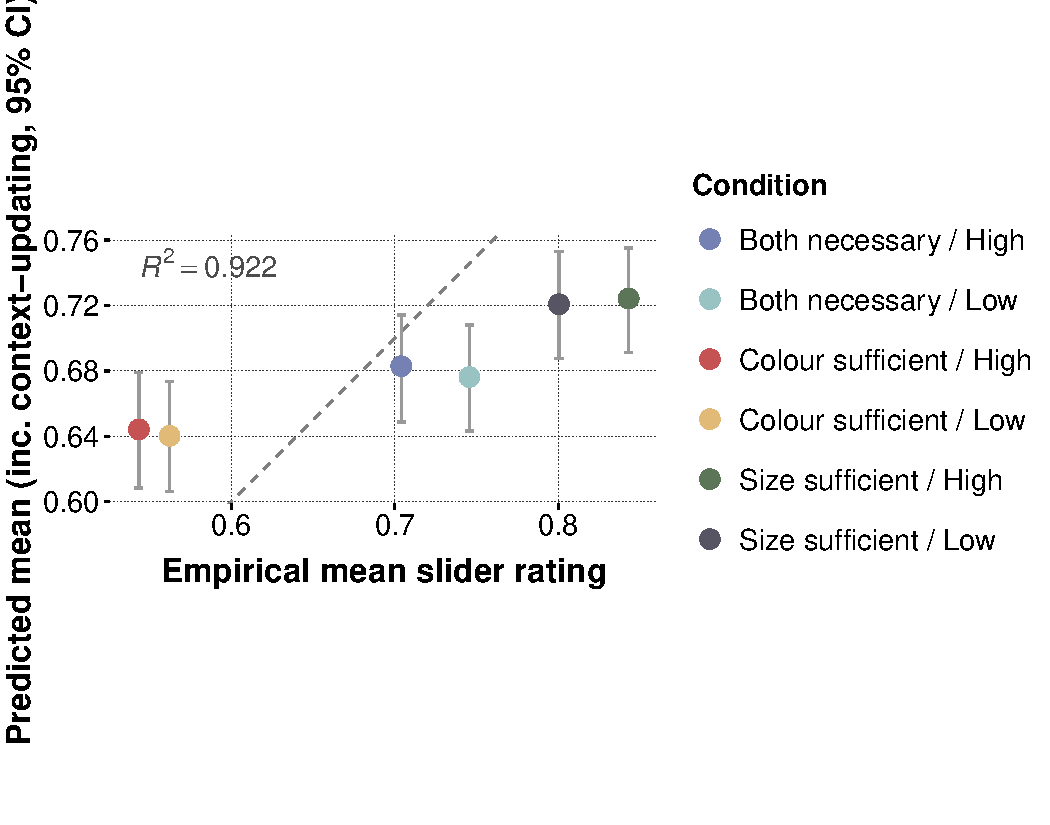
\includegraphics[width=\linewidth]{slider_correlation_inc_hier.pdf}\\[2pt]
    {\small (b) Condition-level correlation}
  \end{minipage}
  \caption{Posterior-predictive fit of the best-fitting slider model (incremental, context-updating).
  (a) Observed (blue) vs.\ model (red) mean slider rating for each referential context $\times$ size-discriminability cell; the dashed line marks no preference ($0.5$) and error bars are $95\%$ confidence and posterior-predictive intervals.
  (b) Observed vs.\ predicted condition means; the dashed line is identity.}
  \label{fig:slider-results}
\end{figure}

\subsection{Free-Production Study}

For production we instantiate the $2 \times 2$ on the extended model of \Cref{sec:model:extended}, with the four cells parameter-matched (\Cref{tab:production-models}): identical ten-parameter inventory, identical participant hierarchy, identical calibrated constants.
The incremental, context-updating cell is the advocated model itself; it reproduces the production data closely ($R^2 \approx 0.94$, $r = 0.97$; \Cref{fig:production-results}, with the by-condition fit in panel~(a) and the condition-level correlation in panel~(b)).
Because the cells differ only in structure, the comparison isolates the speaker architecture and the semantic regime rather than expressive flexibility.

The dominant effect is speaker architecture.
Both incremental cells outperform both global cells by a large margin: the speaker main effect on out-of-sample fit is $+897$ ELPD, and the global cells drop from $R^2 \approx 0.94$ to $R^2 \approx 0.78$.
This effect is not a flexibility artifact.
Under the identical nominal inventory, the effective number of parameters ($p_{\text{LOO}}$) diverges sharply: the incremental cells keep the participant hierarchy identifiable ($p_{\text{LOO}} \approx 145$--$175$ of the 113 participant offsets are data-informed), whereas the global cells collapse it ($p_{\text{LOO}} \approx 7$; the global speaker is too rigid for the data to inform per-participant rationality).
The winning architecture therefore carries the \emph{higher} realized complexity penalty and still wins by $\sim\!900$ ELPD --- its advantage is despite, not because of, flexibility.

Within the incremental pair, the semantic regime now matters: the context-updating cell significantly outperforms the context-fixed cell ($\Delta\text{ELPD} = 63$, dse $= 14$, $|\Delta\text{ELPD}|/\text{dse} = 4.5$).
Within the global pair, the two regimes are effectively tied, with context-updating if anything slightly worse ($\Delta\text{ELPD} = 7$, dse $= 2.6$).
The speaker $\times$ semantics interaction ($+70$ ELPD) is the theoretically informative quantity: context-updating threshold computation adds predictive value, but only when paired with an incremental architecture that can exploit non-commutative composition at each step.
The parameter-matched $2 \times 2$ comparison is shown in \Cref{fig:production-loo}, and the model's posterior-predictive fit in \Cref{fig:production-results}.
Production is thus precisely the setting where word-by-word planning and context-updating semantics jointly matter, consistent with the view that adjective ordering in production reflects online discriminatory utility rather than utterance-level well-formedness alone.

\begin{figure}[htbp]
  \centering
  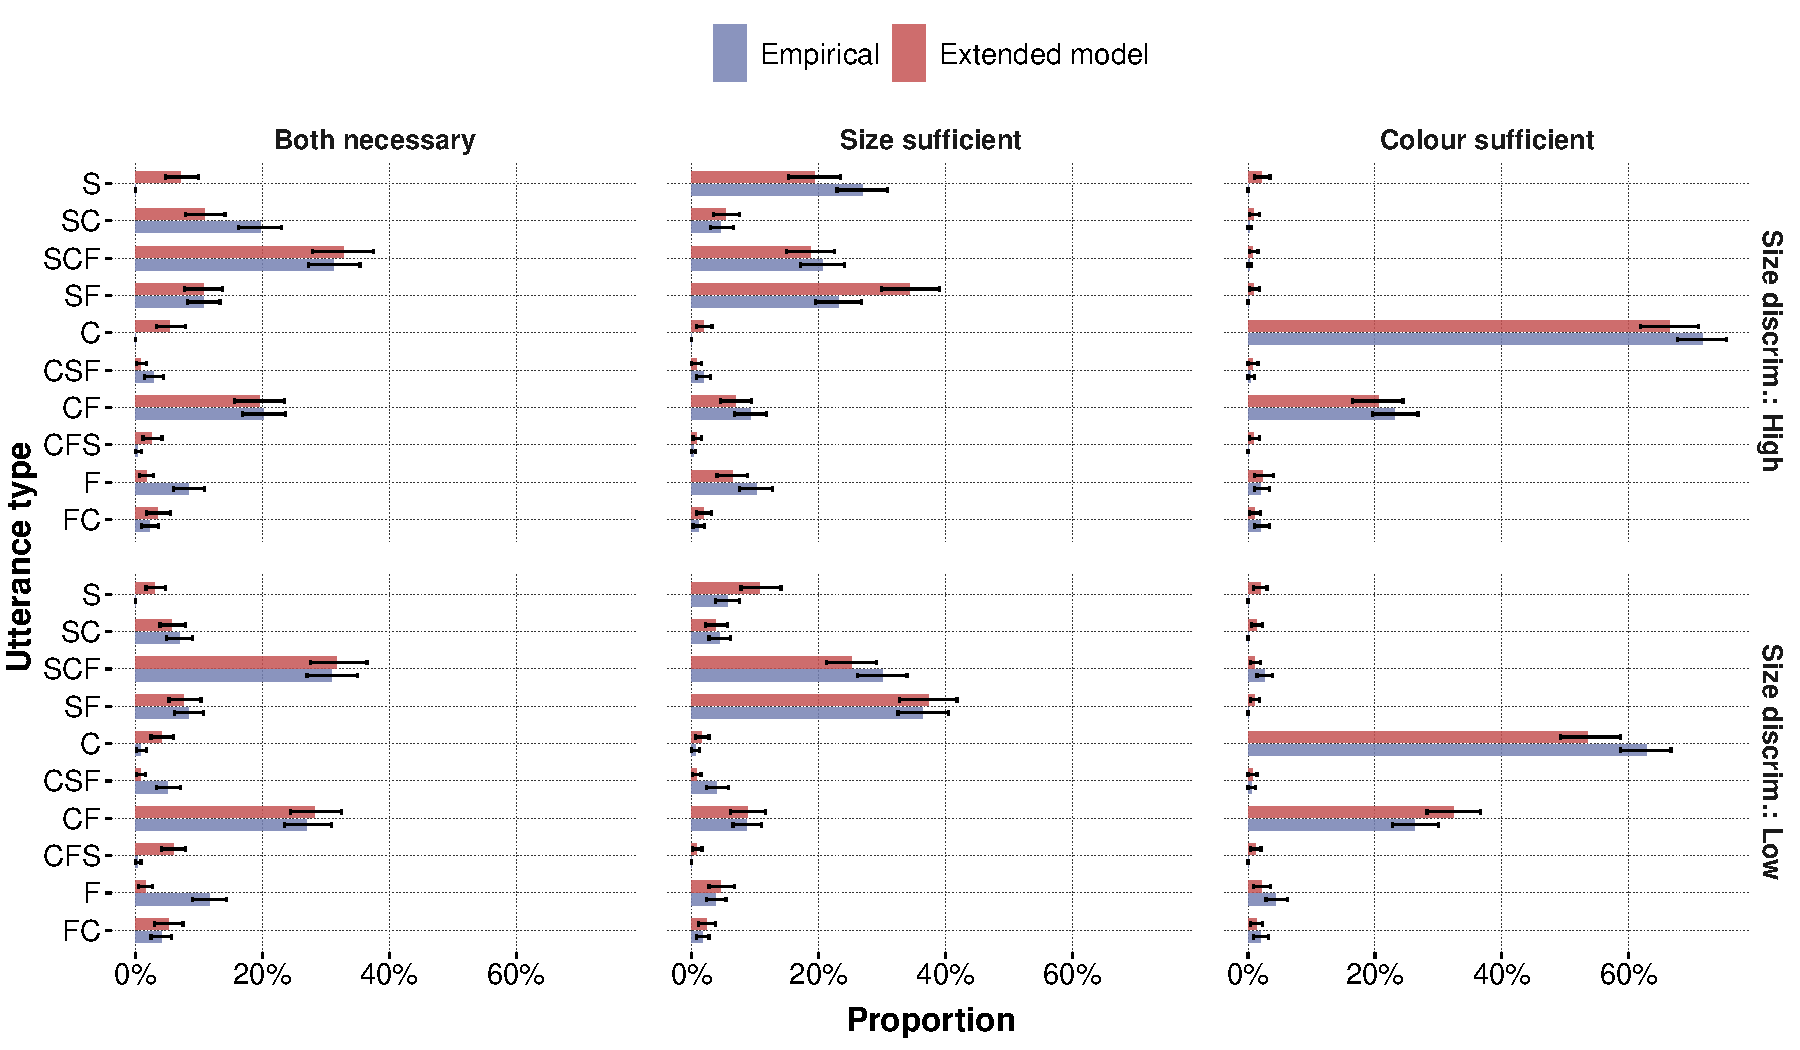
\includegraphics[width=0.95\textwidth]{production_ppc_barplot_best.pdf}\\[4pt]
  {\small (a) Posterior-predictive utterance-type proportions by condition}\\[10pt]
  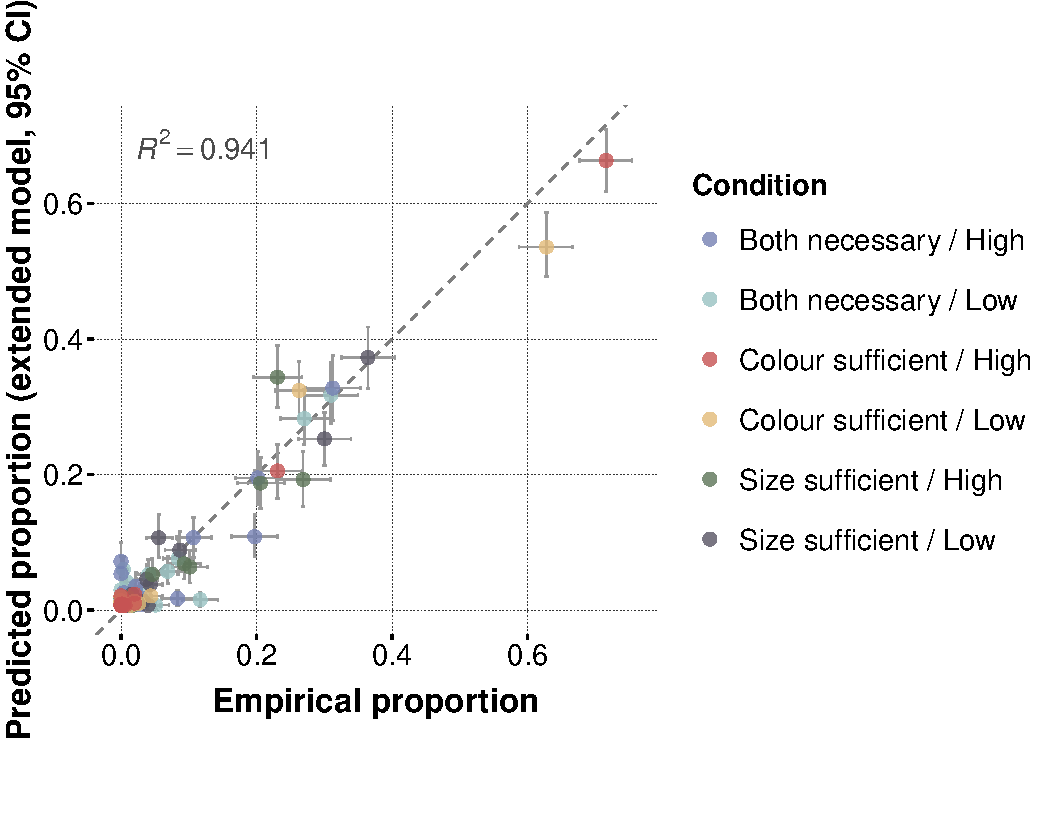
\includegraphics[width=0.62\textwidth]{production_correlation_best.pdf}\\[2pt]
  {\small (b) Condition-level correlation}
  \caption{Posterior-predictive fit of the advocated extended production model (incremental, context-updating; ten parameters, $\nu_\text{colour}=0.59$).
  (a) Observed (blue) vs.\ model (red) utterance-type proportions for each referential context $\times$ size-discriminability cell; error bars are $95\%$ bootstrap and posterior-predictive intervals.
  (b) Observed vs.\ predicted proportions across all condition $\times$ utterance cells ($R^2 \approx 0.94$, $r = 0.97$); the dashed line is identity.}
  \label{fig:production-results}
\end{figure}

The posterior parameters of the advocated (incremental, context-updating) model are reported in full in \Cref{tab:param-inventory}; every $94\%$ HDI excludes zero.
The size and colour informativity weights are well separated ($\alpha_\text{S} \approx 8.0$, $\alpha_\text{C} \approx 3.8$), the canonical colour-before-form penalty is large and tightly estimated ($\lambda_\text{noncanon} \approx 4.4$), and the lapse rate is modest ($\epsilon \approx 0.11$), so little of the fit is absorbed by uniform noise.
The participant-level spread is substantial ($\tau \approx 1.4$), consistent with the high effective parameter count and with genuine individual variability in pragmatic engagement under incremental production.

Three additional ablations of the core incremental speaker are reported in the Appendix.
A lookahead variant, which evaluates both remaining adjective orders before committing to a word, performed worse than the standard greedy incremental model, indicating that local step-by-step planning suffices for this task.
An LM-only ablation, which removes the RSA component and relies solely on the corpus-derived prior, likewise fell short, confirming that the utterance prior alone cannot account for context-sensitive ordering.
An RSA-only ablation, which removes the LM prior, failed the PSIS-LOO diagnostic entirely (high Pareto-$k$ values), suggesting that purely pragmatic choice without a lexical prior produces degenerate predictive distributions for this response space.

\subsection{Cross-Dataset Summary}

Comparing the two datasets reveals a diagnostic interaction between speaker architecture and semantic regime.
Within the incremental models, context-updating semantics significantly improves fit for production ($|\Delta\text{ELPD}|/\text{dse} = 4.5$) but not for slider ratings ($\Delta\text{ELPD} = -0.1$, dse $= 0.2$).
Within the global models, the complementary pattern holds: context-updating semantics provides a massive advantage in the slider data ($\Delta\text{ELPD} \approx 3{,}313$) but confers no benefit in production (a slight decrement, $|\Delta\text{ELPD}|/\text{dse} = 2.6$).
This cross-pattern suggests that context-updating composition is most useful when the model otherwise lacks a source of order-relevant information: in the global slider case, recursive threshold updating is the only mechanism that can break the symmetry between orders; in production, the LM prior already provides ordering information, making the global recursive advantage redundant.
Conversely, when the speaker architecture itself introduces order sensitivity through incremental decision-making, context-updating semantics adds value only when the response space is rich enough (15-way production) to reward finer-grained discriminatory computation.

All models reported in the main text use hierarchical participant-level pooling (random intercepts on the rationality parameter).
Pooled variants, which estimate a single set of parameters across all participants, were consistently worse and are reported in the Appendix.

\begin{figure}[htbp]
  \centering
  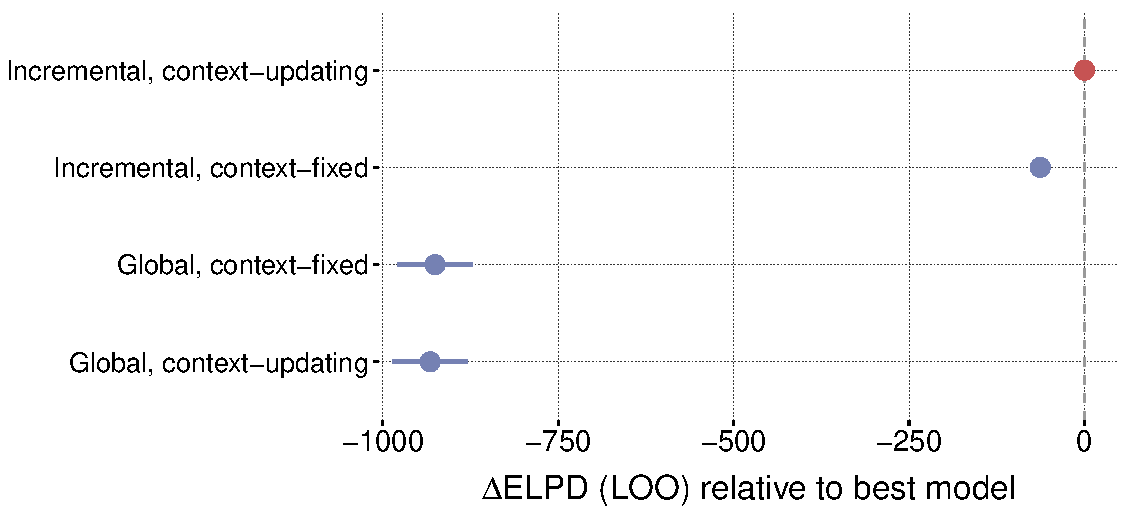
\includegraphics[width=0.7\textwidth]{production_model_comparison_best.pdf}
  \caption{Free-production model comparison: PSIS-LOO $\Delta$ELPD relative to the best cell for the parameter-matched $2 \times 2$ (speaker $\times$ semantics), with $\pm 1$ difference standard error. The incremental cells dominate the global cells (speaker main effect $\approx 897$ ELPD); within the incremental pair, context-updating semantics wins ($|\Delta\text{ELPD}|/\text{dse} = 4.5$).}
  \label{fig:production-loo}
\end{figure}

% =============================================================================
\section{Simulation Study}
\label{sec:simulation}
% =============================================================================

\subsection{Goals and Design}

The simulation addresses three questions that the model comparison alone cannot answer.
First, does the model \emph{generate} a size-first ordering preference across a broad range of contexts, or does this pattern emerge only after fitting to data?
Second, which parameter regions produce a size-first advantage and which, if any, produce a colour-first reversal?
Third, how do speaker architecture and semantic regime jointly determine the ordering preference --- in particular, is context-updating semantics necessary for the baseline effect, or does it emerge from incremental production alone?

To answer these questions, we ran a full factorial sweep over the parameters listed in \Cref{tab:simulation}, crossing both speaker models (incremental, global) with both semantic regimes: recursive (the context-updating regime of \Cref{eq:context_updating}) and static (the context-fixed regime of \Cref{eq:context_fixed}).
Under recursive semantics, the size threshold adapts to the literal listener's running posterior at each composition step; under static semantics, the threshold is computed once from the uniform prior and held fixed.
For each parameter combination, 1{,}000 random six-object contexts were sampled, yielding 12{,}000{,}000 simulated trials in total.
On each trial, the simulation computed the speaker's probability of producing the size-first vs.\ colour-first ordering for the target referent and recorded the size-first advantage (the difference in communicative success between the two orders).

\begin{table}[htbp]
  \caption{Simulation parameter grid}
  \label{tab:simulation}
  \centering
  \begin{tabularx}{0.92\textwidth}{lXl}
    \toprule
    \textbf{Parameter} & \textbf{Values swept} & \textbf{\# levels} \\
    \midrule
    Speaker model & Incremental, global & 2 \\
    Semantics & Recursive, static & 2 \\
    $n_\text{obj}$ & 2, 6, 10, 14, 18, 22, 26, 30 & 8 \\
    $\sigma_\text{spread}$ & 2.0, 7.75, 15.0 & 3 \\
    $\nu$ & 0.90, 0.92, 0.94, 0.96, 0.98 & 5 \\
    $k$ & 0.10, 0.30, 0.50, 0.70, 0.90 & 5 \\
    $w_f$ & 0.1, 0.2, 0.3, 0.5, 0.8 & 5 \\
    \midrule
    Random context samples per combination & 1{,}000 & \\
    \midrule
    \textbf{Total trials} & \textbf{12{,}000{,}000} & \\
    \bottomrule
  \end{tabularx}
\end{table}

The parameter $\sigma_\text{spread}$ controls the spread of the size distribution in the sampled context: low values produce low-discriminability contexts in which size is weakly informative, whereas high values produce high-discriminability contexts in which size strongly separates the target from its competitors.
The remaining parameters ($k$, $w_f$, $\nu$) are the fixed semantic parameters from the fitted models; their individual effects are reported in the Appendix.

\subsection{Results}

\Cref{fig:sim-nobj} shows the size-first advantage as a function of context size and contextual spread, faceted by speaker model (columns) and semantic regime (rows).

\begin{figure}[htbp]
  \centering
  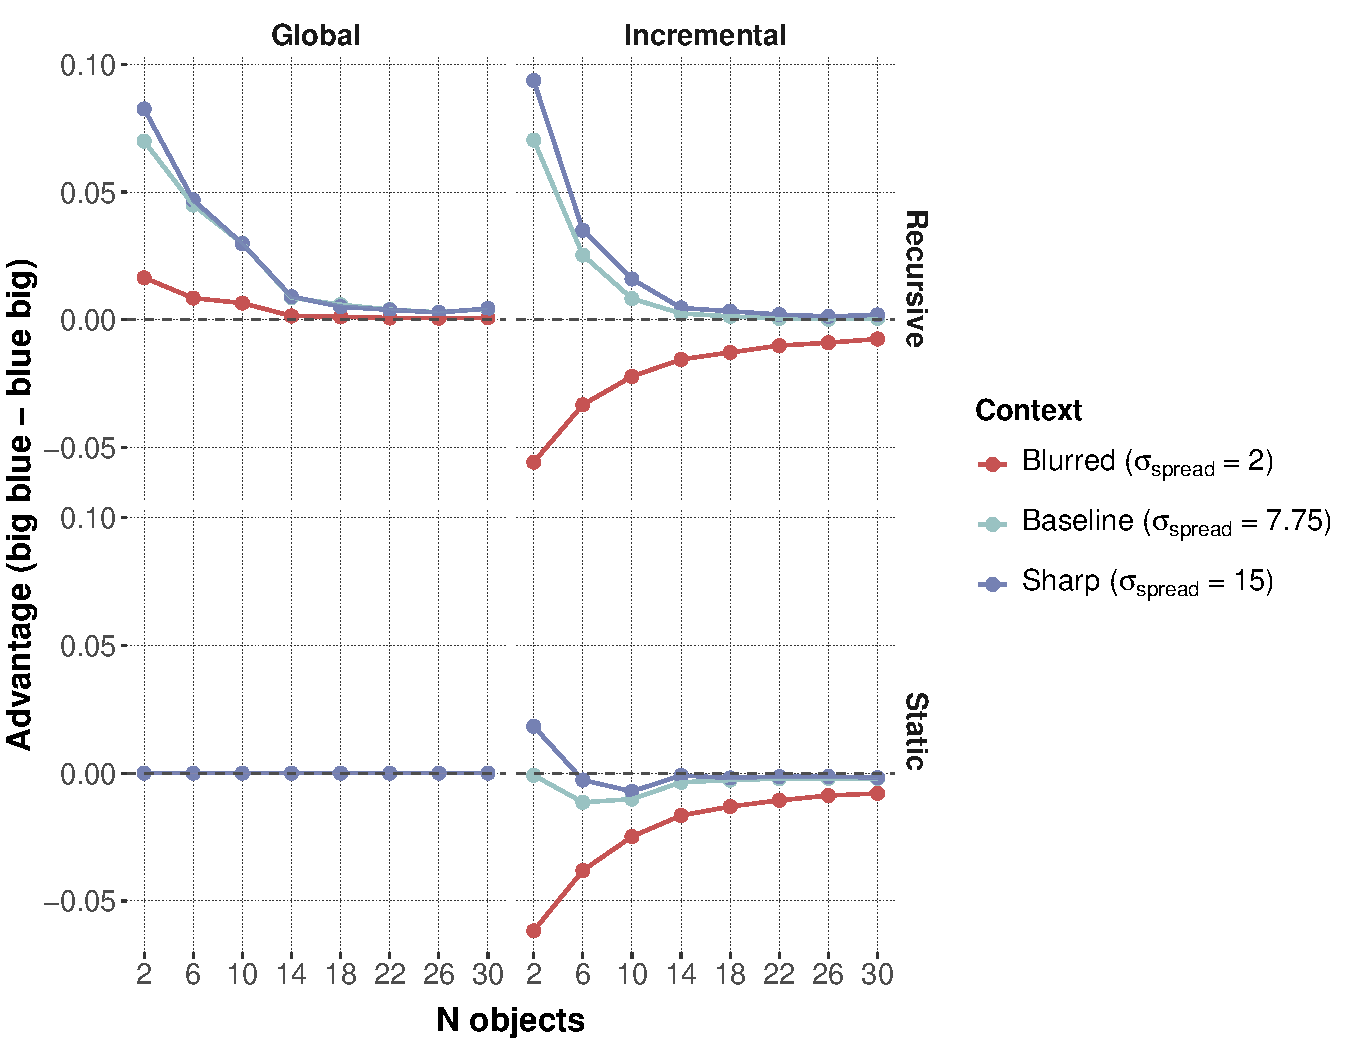
\includegraphics[width=0.90\textwidth]{sim_advantage_nobj.pdf}
  \caption{Size-first advantage as a function of context size ($n_\text{obj}$) and contextual spread ($\sigma_\text{spread}$), faceted by speaker model (columns) and semantic regime (rows). Under recursive semantics (top), both speakers favour size-first order, with the incremental speaker yielding a colour-first reversal in low-discriminability contexts. Under static semantics (bottom), the global speaker produces exactly zero advantage, while the incremental speaker defaults to colour-first.}
  \label{fig:sim-nobj}
\end{figure}

Three findings stand out.
First, under recursive semantics, both speaker models generate a size-first advantage across most of the parameter space.
A global speaker with context-sensitive composition already derives the canonical ordering asymmetry without any incremental machinery.
This result is cumulative with the subjectivity literature: once semantic values are evaluated over progressively restricted comparison classes, less noisy inner modification is sufficient to produce the familiar ordering direction \citep{franke2019subjectivity,scontras2019grammatical,scontras2020incremental}.

Second, static semantics completely eliminates the global speaker's advantage.
Under static semantics, the global speaker produced $\Delta = 0.000$ across all parameter combinations without exception.
When the size threshold does not update during composition, the literal listener assigns identical posteriors to both orderings, making them informationally equivalent.
This reveals that the global speaker's baseline advantage depends entirely on recursive semantics: it stems from order-sensitive threshold adaptation, not from the speaker architecture itself.

Third, the incremental speaker amplifies the size-first advantage under recursive semantics in much of the parameter space and, crucially, generates qualitatively distinct predictions in a specific region: low-discriminability, low-cardinality contexts, where colour-first preferences emerge.
Under static semantics, the incremental speaker defaults to colour-first ($\Delta = -0.009$), driven by the chain-rule asymmetry that favours ``blue'' as the opening token when size is insufficiently diagnostic.
This division of labour clarifies the architecture: context-sensitive composition provides the necessary asymmetry that the global speaker can exploit, while incremental production adds an online control policy whose ordering preference depends on the relative informativeness of each adjective at step~1.

% =============================================================================
\section{General Discussion}
\label{sec:discussion}
% =============================================================================

The present results support a unified view of adjective ordering in referential communication.
Three conclusions stand out.
First, context-sensitive recursive composition is necessary for the baseline ordering effect: the simulation shows that the global speaker produces a size-first advantage only under recursive semantics, where threshold adaptation makes the two orderings informationally non-equivalent; under static semantics the advantage vanishes entirely.
Second, incremental production is the dominant additional mechanism: both incremental models substantially outperform both global models across both datasets.
Third, context-updating semantics and incremental production interact --- context-updating composition adds significant predictive value for production, but only when paired with an incremental speaker.
The full model is not a stack of independent add-ons; its components are synergistic.
These findings connect two strands of the ordering literature that have largely developed in parallel.
The discriminatory-efficiency hypothesis \citep{fukumura2018ordering} predicts that speakers place the most discriminating adjective first, and the empirical modulation of the size-first bias by referential context in both experiments is consistent with this prediction: size-first preferences increase when size is uniquely informative and weaken when colour carries more discriminatory load.
The incremental-efficiency programme \citep{rubio2021wordorder} goes further by proposing that ordering reflects an online production strategy rather than a stored preference, and the dominance of the incremental speaker models in both datasets supports precisely this claim.
What the present model adds is an explicit mechanism linking the two accounts: incremental word-by-word decision-making is the production architecture that allows discriminatory strength to influence ordering in real time, and context-updating semantics is the compositional process that makes discriminatory strength order-dependent in the first place.

The interaction between semantic regime and speaker architecture is the most theoretically informative finding, and also the most nuanced.
Context-updating semantics helps in the production data (15-way choice) but not in the slider data (binary choice), suggesting that the benefit depends on the richness of the alternative space.
Within the global models, the complementary pattern holds in the slider data (context-updating helps) but not in production, where the language-model prior already provides ordering information.
This cross-pattern suggests that context-updating composition is most useful when the model lacks another source of order-relevant information and when the decision architecture can exploit non-commutative semantics step by step.
On the advocated production model the within-incremental advantage of context-updating semantics is decisive ($|\Delta\text{ELPD}|/\text{dse}=4.5$): recursive composition is a genuine synergistic enhancer of incremental production rather than a marginal add-on.

A second methodological point concerns how the speaker $\times$ semantics comparison was made defensible.
The four production cells are parameter-matched: every cell carries the identical nominal inventory, context-fixed is the nested restriction of context-updating, and global versus incremental is a structural switch with no extra parameters, so out-of-sample differences are attributable to mechanism rather than to expressive flexibility.
The realized model complexity ($p_{\text{LOO}}$) is not a nuisance to be matched away but a finding: at an identical nominal inventory the incremental architecture keeps the participant hierarchy estimable while the global architecture collapses it, so the winning model carries the higher complexity penalty and still wins.
This makes the speaker effect conservative rather than inflated, and it is why we treat the speaker $\times$ semantics \emph{interaction}, not a raw fit ranking, as the inferential target.

The calibrated colour semantics is a result in its own right, not just a tuning step.
A near-deterministic colour denotation, assumed a priori, suppresses the pragmatic weight on colour and forces the resulting misfit into a uniform lapse component.
Letting the data choose the colour reliability moves it to roughly $60\%$, which roughly triples the colour informativity weight and halves the lapse rate: the speaker treats colour as a graded, imperfectly reliable cue rather than a categorical one.
This sharpens the relaxed-semantics hypothesis that motivated graded feature denotations in the first place.
It also carries a methodological lesson: a one-dimensional sweep that held the fitted parameters at their old values pointed the wrong way, and only a joint refit that let the other parameters readjust revealed the preferred value.

The production ablation models (reported in the Appendix) further illuminate the division of labour within the incremental speaker.
The LM-only ablation, which strips out the RSA component, performs substantially worse than the full model, confirming that the corpus-derived prior alone cannot account for context-sensitive ordering.
At the same time, the RSA-only ablation, which removes the LM prior entirely, failed PSIS-LOO diagnostics due to high Pareto-$k$ values.
This failure is itself informative: without a lexical prior to anchor the distribution over 15 utterance types, purely pragmatic choice produces degenerate predictive distributions that assign near-zero probability to many attested responses.
The full model thus succeeds because the LM prior provides a well-shaped base distribution that the RSA mechanism reshapes in a context-sensitive direction --- neither component is sufficient on its own.
The lookahead ablation, which evaluates both remaining adjective orders before committing to each word, performed worse than the standard greedy strategy, suggesting that the myopic step-by-step policy is not only simpler but also a better characterisation of how speakers plan in this task.

Three limitations deserve mention.
First, the computational analyses focus on the size--colour subset, although the experiments also included form-based trials.
Consistent with this scope, the parsimony frontier found the RSA informativity weight on form to be uninformative and dropped it: in the size--colour subset, form is produced adequately through the language-model prior, the anchored feature semantics, and the context-gated form-mention boost, without an estimated discriminatory weight of its own.
A fuller account of form as a discriminating feature would require either a stronger justification for treating it as interchangeable with colour or an expanded model fitted to scenes where form carries the referential contrast.
Second, the interaction between semantic regime and speaker architecture differs across tasks, which limits the generality of claims about when context-updating semantics is critical versus secondary.
Tasks with richer alternative spaces may be needed to isolate its contribution more sharply.
Third, the experiments tested only German-speaking participants and only size--colour adjective pairs.
The model's semantic constants were fixed to German-specific values: the language-model prior is corpus-derived, and the colour reliability was calibrated by joint refitting on the German data.
Whether the same architecture generalises to languages with different canonical orderings \citep[e.g., Romance postnominal adjectives;][]{cinque1994,scott2002} or to adjective classes beyond the size--colour pair (e.g., age, material, shape) remains an open question.
Cross-linguistic extension would require both new experimental data and language-specific semantic parameterisation.

Taken together, these results link adjective-ordering research to three traditions that are often discussed separately: subjectivity-based accounts of nominal modification, communicative-efficiency accounts of reference and redundancy, and incremental pragmatic models of language use.
The contribution is not that one tradition replaces the others, but that they can be brought into a single probabilistic framework.
Adjective ordering in referential communication is best understood as a graded adaptation to efficient, incremental reference resolution: subjectivity provides a stable prior over useful orders, discriminatory strength determines how the current scene reshapes that prior, and incremental production with context-updating semantics captures how speakers realise these pressures online.

This characterisation has implications for theories of nominal modification more broadly.
Syntactic accounts that derive ordering from a fixed functional hierarchy \citep{cinque1994,scott2002} correctly predict the default size-before-colour pattern but cannot explain the graded, context-dependent departures observed in both experiments.
Subjectivity-based accounts \citep{scontras2017subjectivity,franke2019subjectivity} provide a principled explanation for the default but treat it as a stable property of adjective classes rather than a context-sensitive outcome.
The present framework subsumes both perspectives: the default ordering arises from the interaction between semantic noise and recursive composition (consistent with subjectivity accounts), while context-dependent modulation arises from the incremental speaker's sensitivity to the current discriminatory landscape (consistent with efficiency accounts).
Future work should test whether this integration extends to adjective classes where subjectivity and efficiency predictions diverge --- for instance, age or material adjectives in contexts where their discriminatory value can be experimentally manipulated.
% =============================================================================
\bibliographystyle{apacite}
\bibliography{references}
% =============================================================================
\appendix
\section{Production Ablation Models}
\label{sec:appendix:ablations}

In addition to the parameter-matched $2 \times 2$ reported in the Model Comparison section, we fitted three ablation variants of the core incremental speaker (single $\alpha$ plus language-model prior, before the extensions of \Cref{sec:model:extended}) to the production data in order to isolate the contributions of specific architectural components.
All ablation models use hierarchical participant pooling.

\paragraph{Incremental lookahead.} Instead of choosing greedily at each word position, this variant evaluates each possible continuation by looking one step ahead and selecting the word that maximizes expected utility over the next two positions.
It tests whether myopic word-by-word choice is sufficient or whether a short planning horizon improves fit.

\paragraph{LM only.} This variant sets the RSA rationality parameter $\alpha = 0$, removing all pragmatic reasoning.
Utterance choice is driven entirely by the language-model prior over word sequences, testing whether phrase-frequency information alone can account for ordering preferences.

\paragraph{RSA only.} This variant sets the language-model weight $\beta = 0$, removing the utterance prior entirely.
All ordering information must come from the RSA informativeness term and participant-level pragmatic strength.
This model was successfully fit, but PSIS-LOO produced non-finite results because a substantial subset of observations have very high Pareto-$k$ values ($k > 0.7$ for 199 of 3{,}196 observations).
This indicates that the leave-one-out posterior is too different from the full posterior for reliable importance-sampling reweighting.
The RSA-only model is therefore excluded from the ranked comparison but is noted here for completeness.

\Cref{fig:ablation-loo} shows the $\Delta$ELPD comparison for the four main models and the two ablation variants with usable PSIS-LOO estimates.
The incremental context-updating model remains clearly best.
The lookahead variant performs worse than both global models, suggesting that greedy one-step choice is more appropriate than short-horizon planning for this task.
The LM-only variant is the worst-fitting model overall, confirming that ordering preferences cannot be reduced to conventional phrase-frequency effects.

\begin{figure}[htbp]
  \centering
  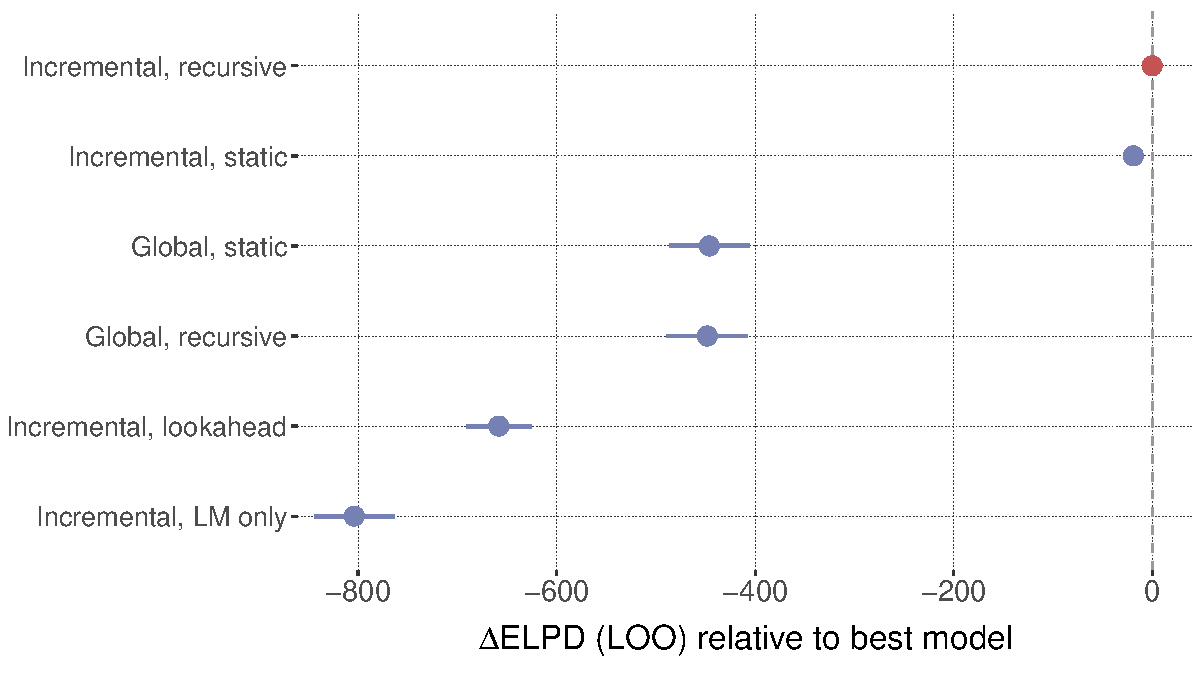
\includegraphics[width=0.75\textwidth]{production_ablation_loo.pdf}
  \caption{Production ablation model comparison. $\Delta$ELPD relative to the best model (incremental context-updating) with difference standard errors. The RSA-only ablation is excluded because PSIS-LOO produced non-finite estimates.}
  \label{fig:ablation-loo}
\end{figure}

% =============================================================================
\section{Extended Production Model: Parameter Inventory}
\label{sec:appendix:inventory}

\Cref{tab:param-inventory} lists the ten population parameters of the advocated production model (\Cref{sec:model:extended}), their priors, and their posteriors at the reference ten-parameter fit.
The participant hierarchy adds 339 latent offsets (113 participants $\times$ 3 conditions) drawn from a zero-mean normal with standard deviation $\tau$.
The fixed constants are $\nu_\text{colour}=0.59$, $\nu_\text{form}=0.50$, $k=0.50$, $w_f=0.69$, and the language-model temperature fixed at its stable posterior median.
The posteriors below are from the reference fit ($\nu_\text{colour}=0.97$), at which every coefficient is documented; under the calibrated $\nu_\text{colour}=0.59$ the four most colour-sensitive coefficients shift as reported in the main text ($\alpha_\text{S}\!\approx\!8.0$, $\alpha_\text{C}\!\approx\!3.8$, $\lambda_\text{noncanon}\!\approx\!4.4$, $\epsilon\!\approx\!0.11$), and every $94\%$ HDI continues to exclude zero.

\begin{table}[htbp]
\centering
\caption{Population parameters of the advocated production model: prior and posterior mean with $94\%$ HDI at the reference ten-parameter fit.}
\label{tab:param-inventory}
\small
\begin{tabular}{llll}
\hline
Parameter & Role & Prior & Posterior \\
\hline
$\alpha_\text{S}$ & RSA informativity weight, size & HalfNormal$(5)$ & $6.24\;[6.02,\,6.48]$ \\
$\alpha_\text{C}$ & RSA informativity weight, colour & HalfNormal$(5)$ & $1.26\;[0.95,\,1.58]$ \\
$\lambda_\text{suff}$ & first-word boost for the sufficient dimension & Normal$(0,1)$ & $1.58\;[1.19,\,1.97]$ \\
$\lambda_\text{form-mod}$ & context-gated form-mention boost & Normal$(0,2)$ & $2.82\;[2.62,\,3.05]$ \\
$\lambda_\text{noncanon}$ & form-before-colour penalty & HalfNormal$(2)$ & $2.82\;[2.21,\,3.46]$ \\
$\gamma_\text{base}$ & base per-word length bias & Normal$(0,2)$ & $3.10\;[2.94,\,3.26]$ \\
$\gamma_\text{one}$ & length modulation when one word suffices & Normal$(0,2)$ & $-2.37\;[-2.57,\,-2.19]$ \\
$\gamma_\text{sharp}$ & extra length under perceptual blur & HalfNormal$(2)$ & $0.68\;[0.53,\,0.82]$ \\
$\epsilon$ & lapse / uniform-noise rate & Beta$(1,50)$ & $0.18\;[0.17,\,0.20]$ \\
$\tau$ & SD of participant rationality offsets & HalfNormal$(0.2)$ & $1.35\;[1.12,\,1.59]$ \\
\hline
\end{tabular}
\end{table}

% =============================================================================
\section{Simulation Parameter Sweeps}
\label{sec:appendix:sim-params}

\Cref{fig:sim-k,fig:sim-wf,fig:sim-csv} show how the three fixed semantic parameters affect communicative success across the two speaker models.

\begin{figure}[htbp]
  \centering
  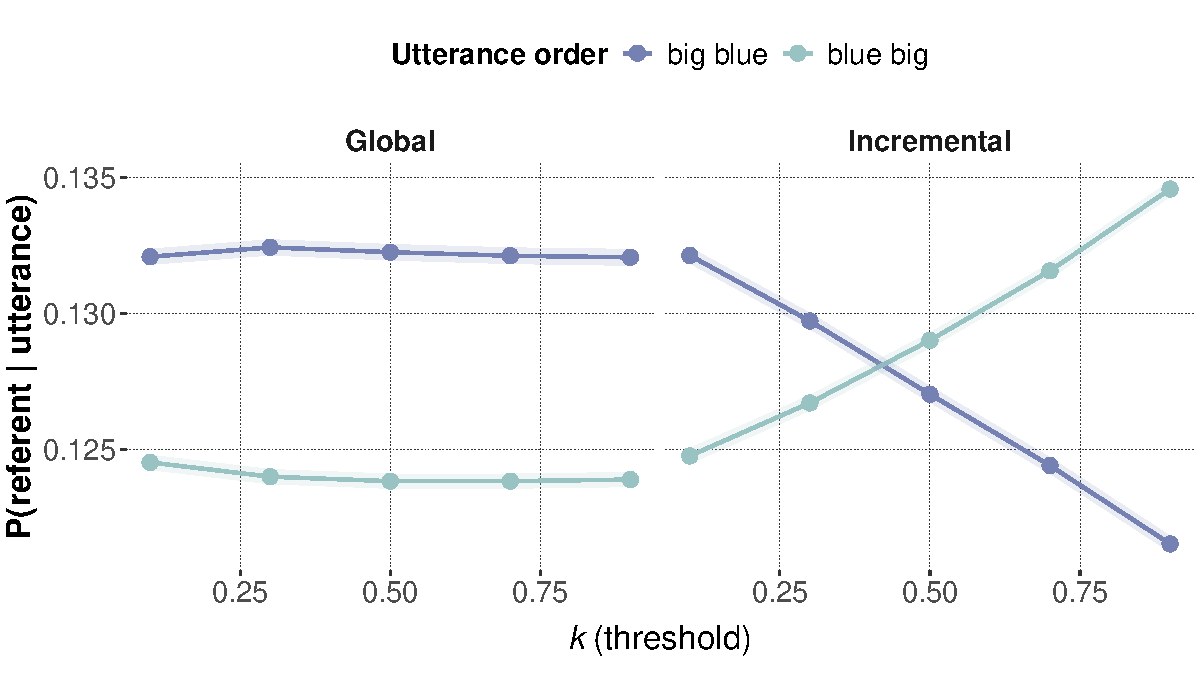
\includegraphics[width=0.86\textwidth]{sim_k.pdf}
  \caption{Effect of the threshold parameter $k$ on communicative success in the simulation. Lower values of $k$ make the size threshold more restrictive and reduce the success of both orderings, while preserving the incremental speaker's size-first advantage.}
  \label{fig:sim-k}
\end{figure}

\begin{figure}[htbp]
  \centering
  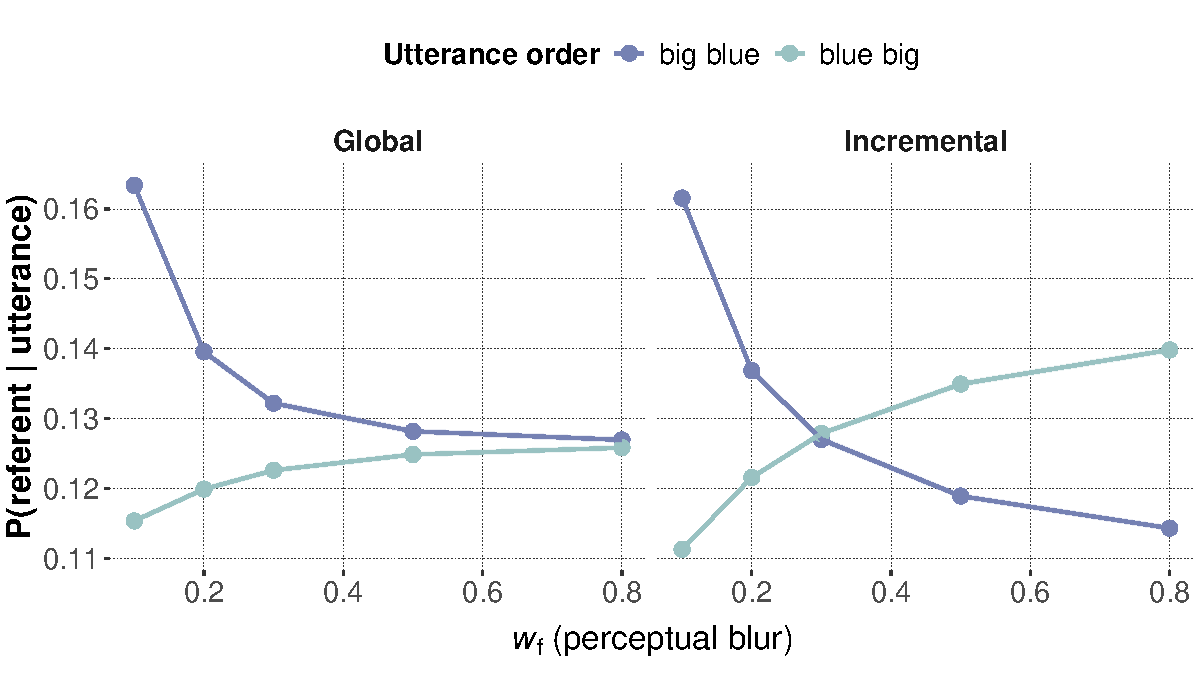
\includegraphics[width=0.86\textwidth]{sim_wf.pdf}
  \caption{Effect of perceptual blur $w_f$ on communicative success in the simulation. As blur increases, the advantage of size-first ordering decreases, especially for the global speaker.}
  \label{fig:sim-wf}
\end{figure}

\begin{figure}[htbp]
  \centering
  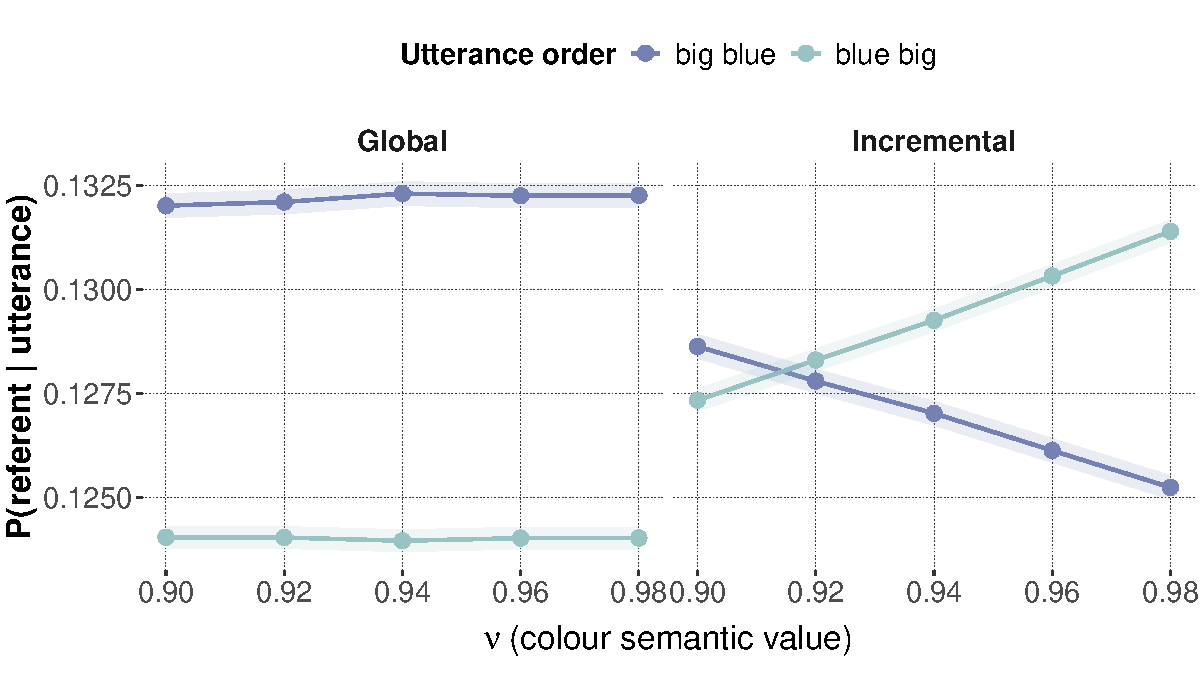
\includegraphics[width=0.86\textwidth]{sim_colorsemval.pdf}
  \caption{Effect of the colour/form semantic value $\nu$ on communicative success in the simulation. Higher values of $\nu$ make feature adjectives more deterministic and reduce the relative size-first advantage.}
  \label{fig:sim-csv}
\end{figure}

\end{document}
